\documentclass[]{usiinfbachelorproject}
\usepackage{subfig}
\usepackage{caption}
%\usepackage{subcaption}
\usepackage{float}
\usepackage{listings}
\usepackage{graphicx}
\captionsetup{labelfont={bf}}

%\newcommand\subsubsection{\@startsection{subsubsection}{3}{\z@}%
%                {-3.25ex\@plus -1ex \@minus -.2ex}%
%                {1.5ex \@plus .2ex}%
%                {\normalfont\normalsize\bfseries}}
%\newcommand\paragraph{\@startsection{paragraph}{4}{\z@}%
%                {3.25ex \@plus1ex \@minus.2ex}%
%                {-1em}%
%                {\normalfont\normalsize\bfseries}}
\author{Francesco Saverio Zuppichini}

\title{Design Interactive Display Applications}
\subtitle{for Active and Walk-by Contact Personalization}
\versiondate{\today}
\begin{committee}
%With more than 1 advisor an error is raised...: only 1 advisor is allowed!
\advisor[Universit\`a della Svizzera Italiana, Switzerland]{Prof.}{Marc}{Langheinrich}
%You can comment out  these lines if you don't have any assistant
\assistant[Universit\`a della Svizzera Italiana, Switzerland]{}{Dr. Ivan}{Elhart}
%\assistant[Universit\`a della Svizzera Italiana, Switzerland]{}{AssistantName2}{AssistanSurname2}
\end{committee}


\abstract {
Nowadays the majority of public displays follow a closed model by showing static and passive content. People have started to ignore them due to their low utility. Opening them to interactive applications that support user personalisation could create a new communication channel for the 21st century. 
In the last years, the interest into this field has increased leading to the development of different systems that uses digital signage to deliver personalised content. 

Our project takes inspiration from previous researches, creating a new architecture that allows users active and walk-by content personalisation. Active contact personalisation allows the viewers to temporally take control of the screen using a mobile application. Walk-by personalisation is the possibility to access the personalised content by  walking to nearby a display.  Our system is composed by five elements: \emph{Map Provider}, a \emph{Proxy}, \emph{Mobile Application} and two display interactive applications:\emph{Transport} and \emph{Upcoming Classes}. In this project we present our prototype implementation of the architecture, the design study and an overview of its main functionalities. 
}


\begin{document}
\maketitle

%%%%%%%%%%%%%%%%%%%%%%%%%
\tableofcontents
\newpage
\section{Introduction}
\subsection{Motivation}

Public displays have emerged as a widely used mass communication channel in the last years. They are commonplace in public places such as squares, supermarket, and in our case, universities. 
Traditionally they were used as a common broadcast medium pushing static and passive content to the audience adopting a closed model. Nowadays, this model is still the most used. This approach can be observed in Figure 1 (a) that shows the New Yorks Times Square while (b) paints the same city in the later half of the 20th century. It can be noticed that displays and posters are used for the same goal: advertisement.

Due to a decreasing of people's interest towards them, displays stakeholders have tried a different approach to gather back the audience's attention. One of the most common is to just increase the number of screens. This strategy has lead to a ubiquitous deployment of public displays making viewers ignore them even more.
\begin{figure}[H]
  \centering
  \subfloat[Times Square]{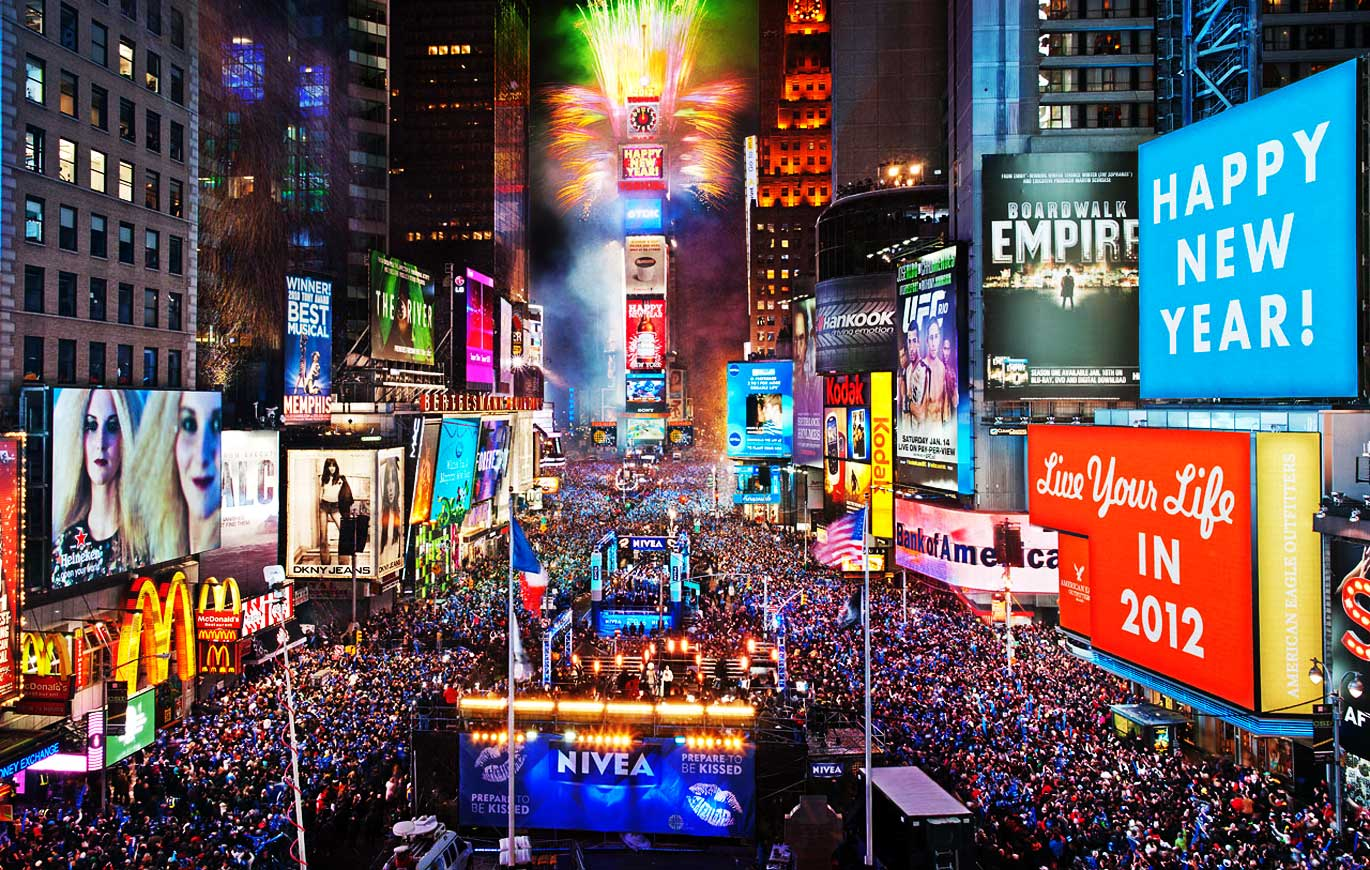
\includegraphics[width=0.5\textwidth]{./images/new_york_displays.jpg}}
  \hfill
  \subfloat[New York in the 60s]{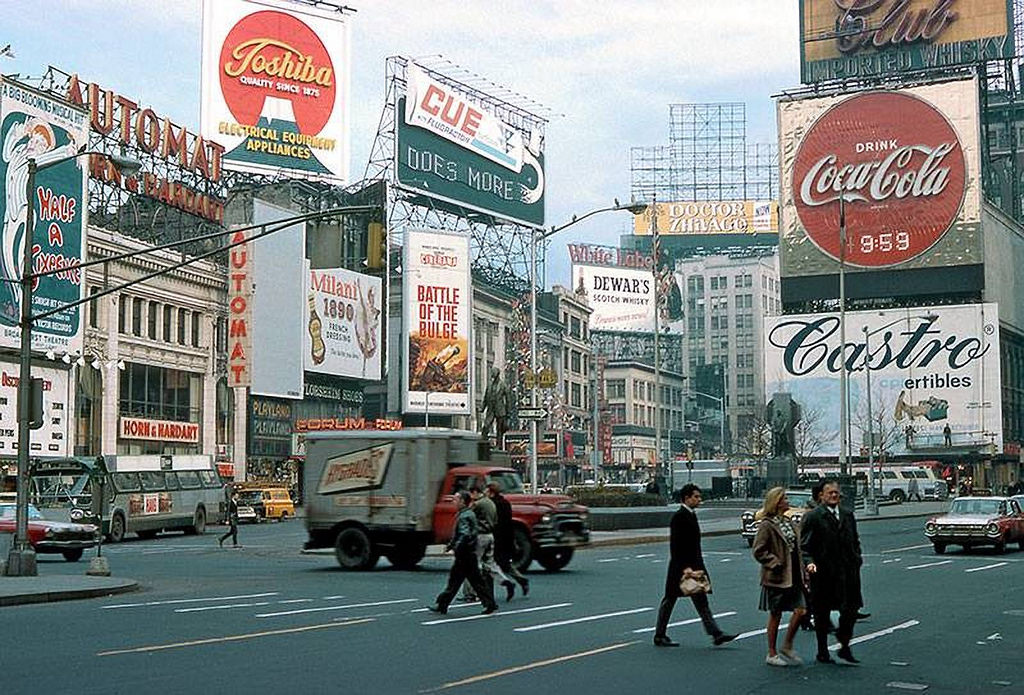
\includegraphics[width=0.46\textwidth]{./images/new_york_posters.jpg}}
  \caption{Example of public displays}
\end{figure} 
The major problem is the lack of users personalisation. In the last years, the interest in this field increased and lost of studies were proposed in order to solve the problem. Recently, researches have developed system where the users can ask the displays through a mobile application to show custom content such as map, transit timetables or schedules. Most of them follow the Mark Weiser's \cite{the_computer_for} vision in which computers becomes part of the environment disappearing by fading in the background.
Some examples may be the \emph{e-Campus} \cite{e_campus} in the University of Lancaster that shows interactive content such as Youtube videos, \emph{USI Display} \cite{a_good_balance} used in the \emph{Universita della Svizzera Italiana} where students can access an array of campus' applications, PriCal \cite{pri_cal} an ambient calendar display that displays a user's schedule and \emph{Instant places} \cite{pins_and_posters} where users can pin their favourite soccer team.
By taking advantages of the last technologies advancements, that had brought the touch interface to the displays, we can create interactive applications that allow users to surf content directly on the display making them more attractable.

Our project aims to design an architecture that supports interactive displays' application and active and walk-by contact personalisation.
Active contact personalisation allows the viewers to temporally take control of the screen deciding which content will be shown on the screen by selecting preferences through a mobile interface. Walk-by personalisation is the possibility to access the personalised content by by just walking nearby a display thanks to Bluetooth beacon's places nearby them. This gives an array of advantages, for instance, the viewers can select their content once and just walk to display when he needs it. Moreover, public displays are usually placed in very accessible places making even easier for the audience to find them. 

Usually, public displays  \emph{"have [...] been investigated from the perspective of single user
interaction paradigm"} \cite{personalisation_and_privacy}. In this model, a user can access a rich array of applications and services from the screen. However, since public displays are used by a homogenous audience, multi-user support must be the provider. In our project, we support both single user and multi-user model by taking advantages of GUI techniques to improve the services' accessibility. One interested case study was conducted in this university \cite{design_considerations} where emerged the importance of using a clear design for both a mobile application and display  \emph{"so that people may associate the content they see on the displays with the application generating that content"} \cite{design_considerations}

Other studies in this field demonstrate the important of user's privacy in pervasive display networks. A solution was proposed \cite{personalisation_and_privacy} to solved the problem by creating an architecture that \emph{"support displays personalisation without allowing a display network to track and profile users views"}.
In our project, we took inspiration from these researches in order to also make users' preferences anonymous by using a colour based approach in the system so no other viewers can know whose preferences are. 
 
\subsection{State of the Art}
User users personalisation in pervasive display networks is not a new idea. A number of previous projects have been suggested in order to solve the lack of users interactions. However, \emph{"only a small number of them supports multi users and multi displays"} \cite{a_good_balance} stakeholders, such as \emph{e-Campus} \cite{e_campus}, \emph{Usi Display}, \emph{PriCal} \cite{pri_cal} and \emph{Instant Places} \cite{pins_and_posters}.

\emph{e-Campus} is a wide public displays network in Lancaster University that supports interactive application such as Youtube, Flicker and campus-based information visualisation \cite{e_campus}.The system counts thirty displays representing a successful example for our project.

\emph{USI Displays} is the current architecture used by \emph{Universita della Svizzera Italiana} \cite{a_good_balance}. The network supports a range of applications that focus on providing useful information to the faculty student. For example, it is possible to get information about bike sharing, exams or public transportation. One limitation is the lack of users preferences.

\emph{PriCal} is a smart interactive calendar display application \cite{pri_cal}. The main idea is to let the audience see their schedules directly into the display. A context-adaptive privacy is provided by detecting the viewers and adapting their events visibility according to their preferences. An interesting aspect of this project is the architecture implementation. Their system supports both registered users as well as unknown persons providing a quality network and facilitates interaction by passers-by. 

\emph{Instant Places} is a web-based display platform using the metaphors of Pins and Posters \cite{pins_and_posters}. In their study, they created an \emph{"application that displays content associated with the soccer teams supported by place visitors"} \cite{pins_and_posters}. A pin is created for each team and when a user selects it, the displays shows associated content. At the same time, the application displays a global view of others selected pins giving a feedback to the user about people's preferences.

%\subsection{Goal}
%
%The goal of this project is to develop an architecture that supports active and walk-by contact personalisation by creating two new interactive displays' application: \emph{Transport} and \emph{Upcoming Classes}.
%both of them must supports users preferences by exposing a common UI mobile interface to manage them.
%
%The first one aims to provide a convenient way to navigate and discover busses schedules. Also using geo localisation to also display directions to nearby stations to the viewer.
%
%\emph{Upcoming Classes} shows the semester schedule to the faculty's student by also
%
%
%The architecture must provide a mobile application to manage users information, access interactive applications and discover nearby displays using Bluetooth beacons.
%
%Since we are targeting a heterogeneous audience, the content must be easily accessible. So, we focus our attention to the UI design aimed to provide a natural flow of interaction between the system and each interactive application.
%
%Moreover, the architecture must be scalable in order to allow future developers to extend our project by adding, for example, new applications to the displays. 

\subsection{Results}
With our project, we created a network that supports users personalisation into public displays by developing a new architecture with two interactive applications. The audience can see their preferences by just walking nearby a screen while interacting with the mobile application that may also run in background. Furthermore, information can be retrieved directly from the display using a touch interface. For instance, is possible to see buses' schedules by clicking on a station. In order to store the state of displays, applications and beacons, a \emph{MAP Provider} were developed. It exposes a web socket is used to broadcast real-time notification through all the system notifying the presence of a user near a screen.

The applications developed are \emph{Transport} and \emph{Upcoming Classes}. \emph{Transport} allows users to select their bus schedules as preferences and access useful content directly on the screen, like see directions from the display to the stations.
\emph{Upcoming Classes} shows the semester schedules supporting custom queries in order to discover specific content. A colour based approach is used to identifier users' preference by only the creator. The user can select a custom colour in the mobile application that will be showed in the display.

\section{Architecture}
\subsection{Overview}
Our system is composed by five elements: \emph{Map Provider}, a \emph{Proxy}, \emph{Mobile Application} and two display's interactive applications. These applications are: \emph{Transport} and \emph{Upcoming Classes}. The components communicate using REST calls and Web Sockets that are proxied to the clients in order to serve all the applications from the same domain as is showed in Figure 2. Each of them exposes an API that can be called in order to get the required data in JSON format.

The \emph{Map Provider} stores the state of displays, beacons, users and the applications' information with the purpose of making them available to the system. A web socket is used to broadcast real-time notification through all the clients to provide real-time feedback about the global network state.

We developed two display's application, \emph{Transport} and \emph{Upcoming Classes}, using the same common interface abstracting them into the \emph{Application Layer} (Figure 3). It is possible to individually add new applications by making them conform to our API interface for preference personalisation. Therefore, each application can be added from everywhere allowing developers to use their favourites technologies and hosting platforms.
Since they follow a common structure, we will refer to them as the \emph{Application Layer}.

A simple \emph{Proxy} is used to forward both HTTP request and web sockets for serving each applications from the same Domain avoiding cross-origin requests. Our network supports both HTTP and HTTPS, for security reason, the sockets only work in secure mode.
\begin{figure}[H]
  \centering
  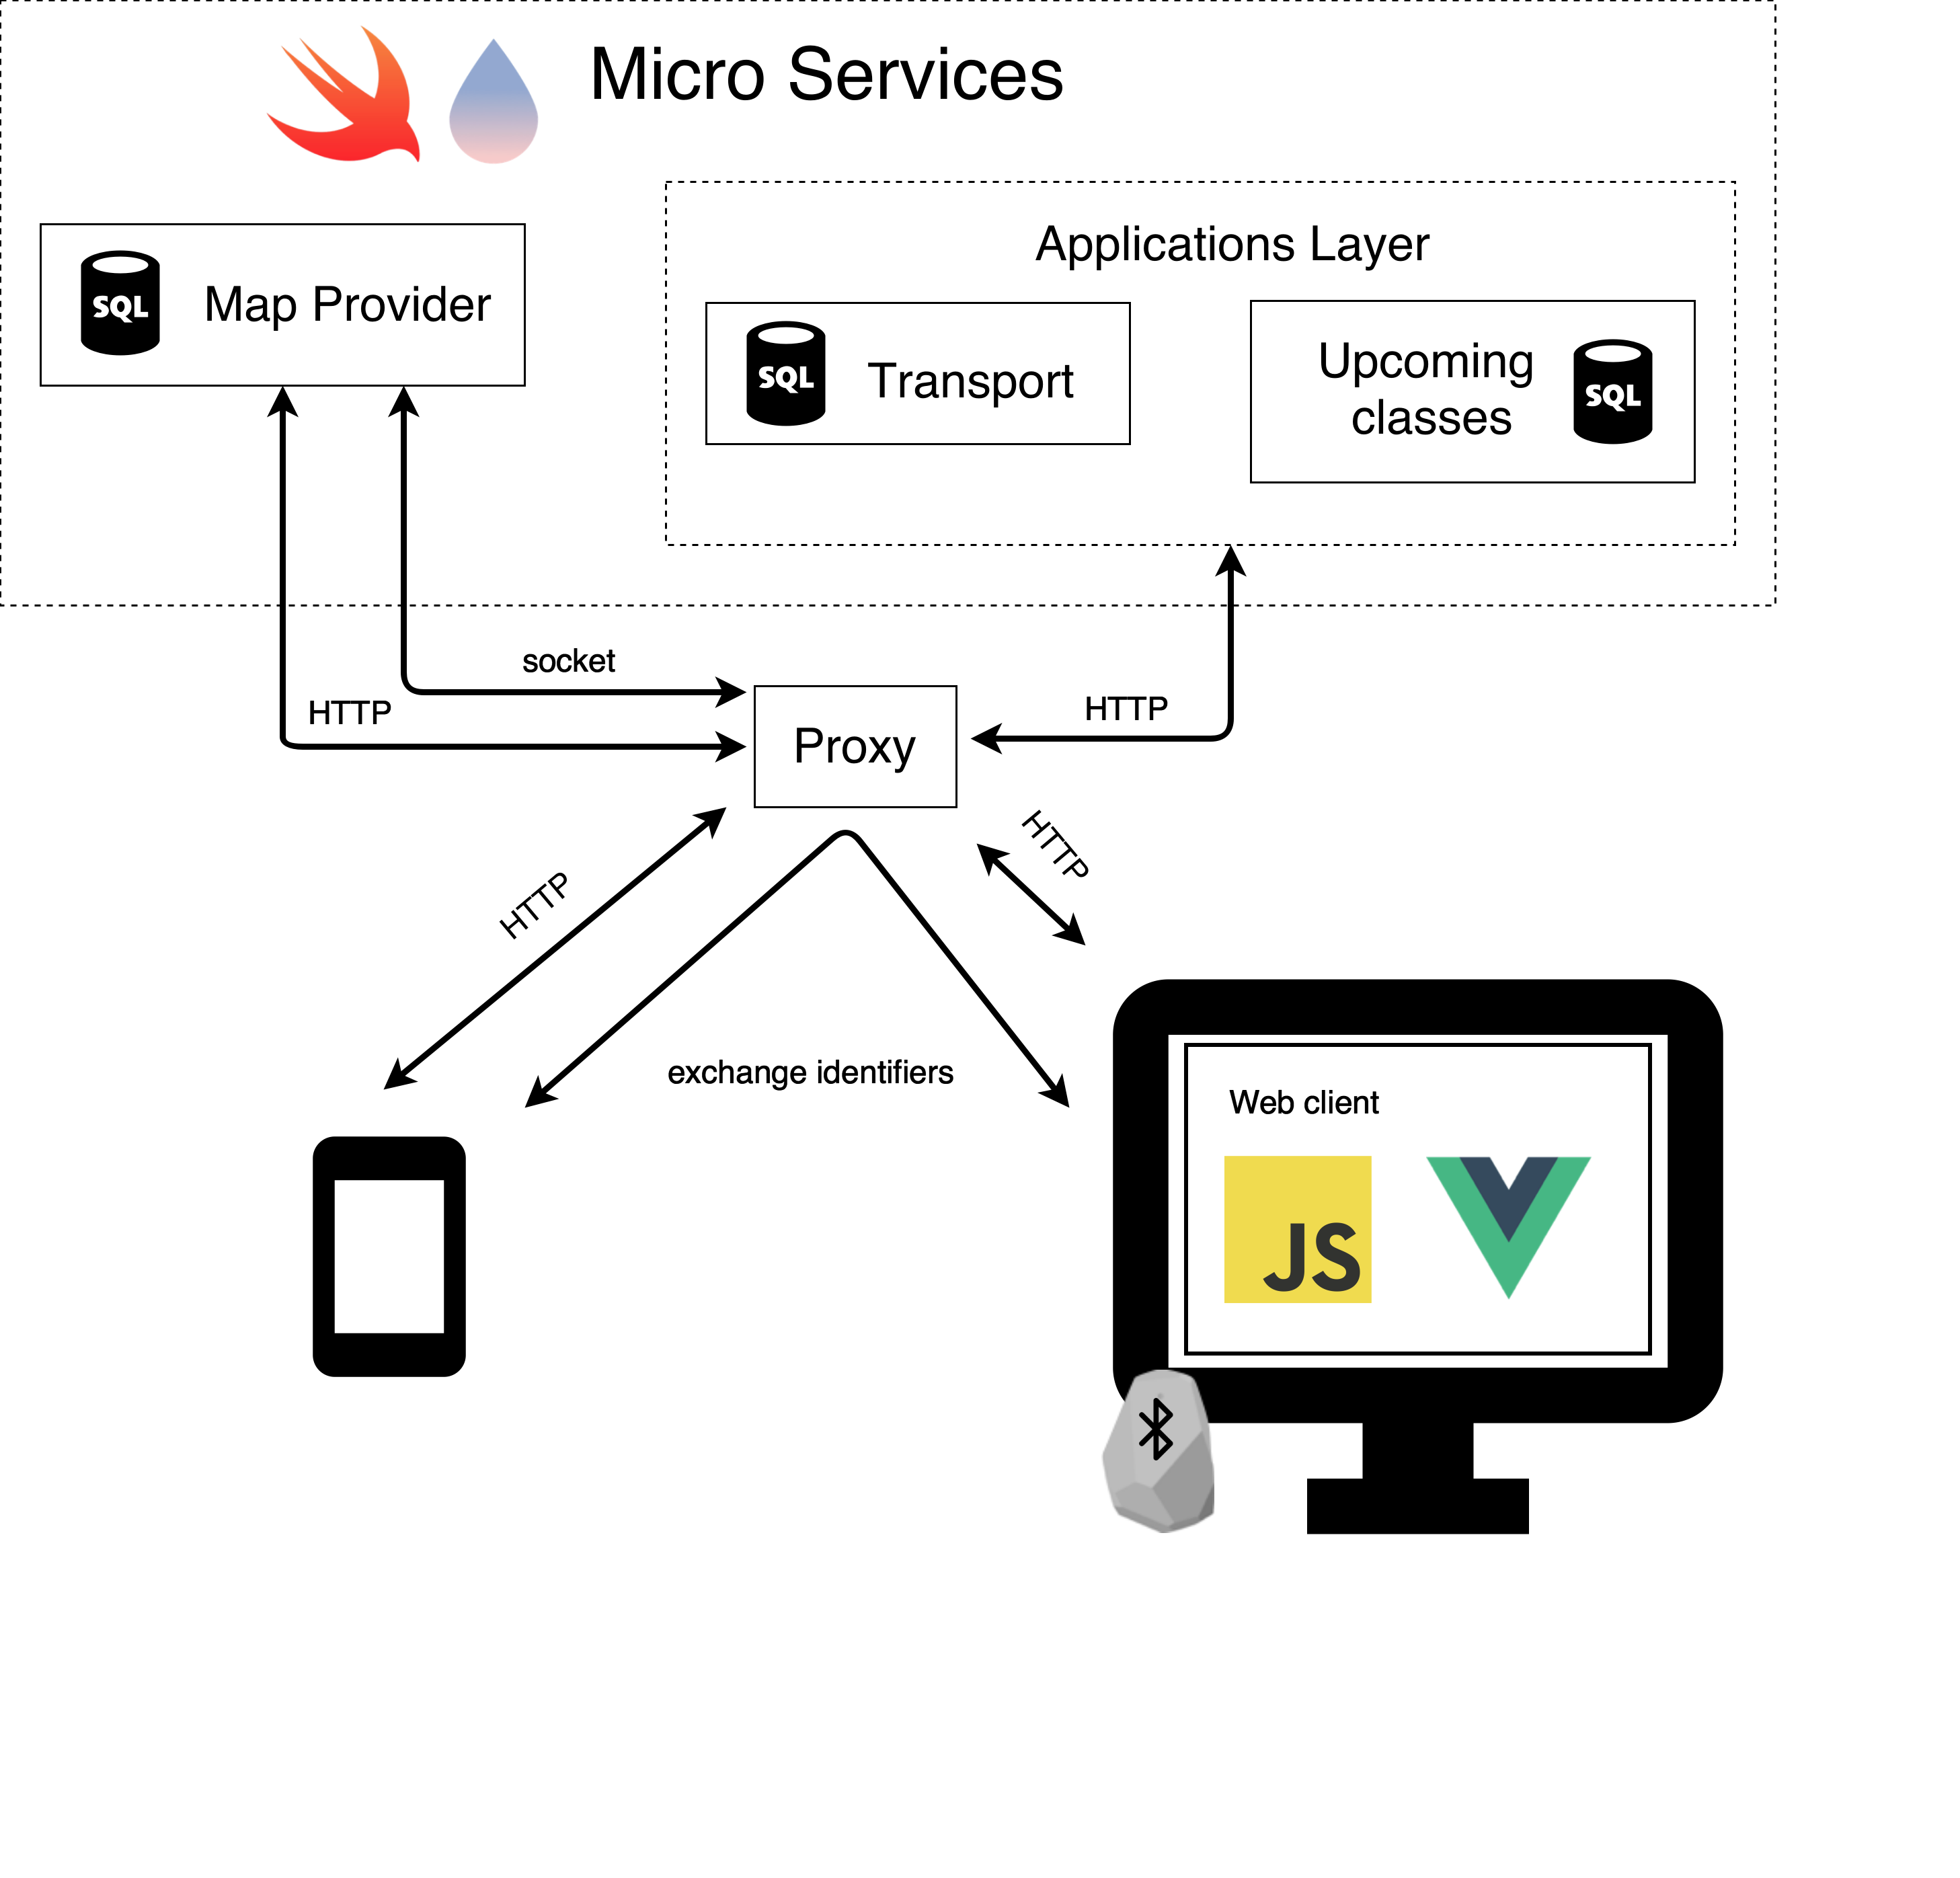
\includegraphics[width=0.9\textwidth]{./images/poster_image_1.png}
    \caption{Architecture Elements}
\end{figure} 


% TALK about the system that must be anonymous 
%
\subsection{Architecture Elements}
\subsubsection{Map Provider}
The \emph{Map Provider} stores in a database information about displays, beacons and available applications in order to make it possible for the client to access to the \emph{Application Layer} and have a global knowledge of the current network state. A many to one relation is created between the Display table and the Application table(Figure 3), since a single screen can run multiple application at the same time. In our project we limited to one main application for screen, but, using a responsive design approach, it is possible to maintain a pleasant look even if one is shrunk due to displays size limitation. Since the \emph{Map Provider} allows to enable and disable custom services, a many to many pivots is used to keep track of local user's applications state. If an application is turned off and a user is near to a display running that application, then no interaction between the two will happen. In our design, this check, is done on the mobile application in order to send fewer information into the socket.

The physical device that makes the in-walk communication possible is the Bluetooth beacon produced. They are produced by Estimote. A many to one relation between Beacon and Display table is used to identify a display thought a beacon's id. In our design, many beacons can be linked to the same screen, but two or more displays cannot have any beacons in common. The model stores the beacon's mac address as unique identifier. These devices must be put really close to the machine we want to identify to accomplish better location accuracy. Moreover, thanks to our API design, they can be changed at any time by just sent the correct request to the server. 
A User table is stored with basic information such as email and favourite colour. With the mobile application is possible to enable and disable applications to prevent information flow to them. To keep track of those preferences, a one to many relation from User and Application table is stored. 
\begin{figure}[H]
  \centering
  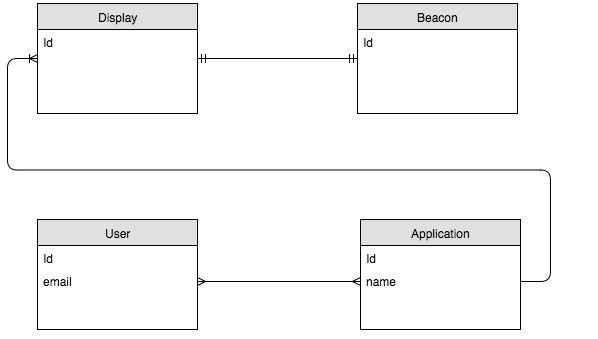
\includegraphics[width=0.55\textwidth]{./images/TacitaRelations.jpg}
   \caption{Relations in the Map Provider}

\end{figure} 

\subsubsection{Transport App}
The \emph{Transport} application allows users to navigate the nearby bus station and create preferences through the mobile interface. We decided to gather the data from the well designed Opendata API (https://transport.opendata.ch/) that allows fetching all kind of transportation information, in our case buses.
However, due to the limit number of request we can make, fixed to three per second, and the necessity to have some custom endpoint, we cloned them.

We also have integrated Google Maps API into the screen's front-end. So, after fetching the exactly display's position thanks to web browser geo localisation, we can show the estimated time to get to a specific station by walk and the correct directions. With this information we can give real-time visible feedback on screen when it is going to be too late to catch a specific bus. Since we are using a built-in web browsers feature, we can easily scale our system. The image you need to move the display to one location to another, with our architecture there is no need to update its state into the server. Since the information is fetched client side, its position is updated as soon as it is moved, as well as with all the other functionalities related to it,  no external operation is needed.

Even if it can be argued that by cloning Opendata API we loose all information about transports delays, we notice that the delay field is always null. So, we have to assume that even them can not have access to such detailed information or it is not implemented yet. For our project, we cloned them every 6 hours, but the schedule can be changed in virtual no time. A mobile interface was implemented to to create, edit and remove preferences. To do so, the user must select the correct station, buses and direction. Figure 4 shows how a preference is created. From left to right, the user presses a floating button and selection station page appears. Using a step by step approach the preference is created, and, after confirming the creation in the modal, it is added to the user's preferences.  

\begin{figure}[H]
  \centering
  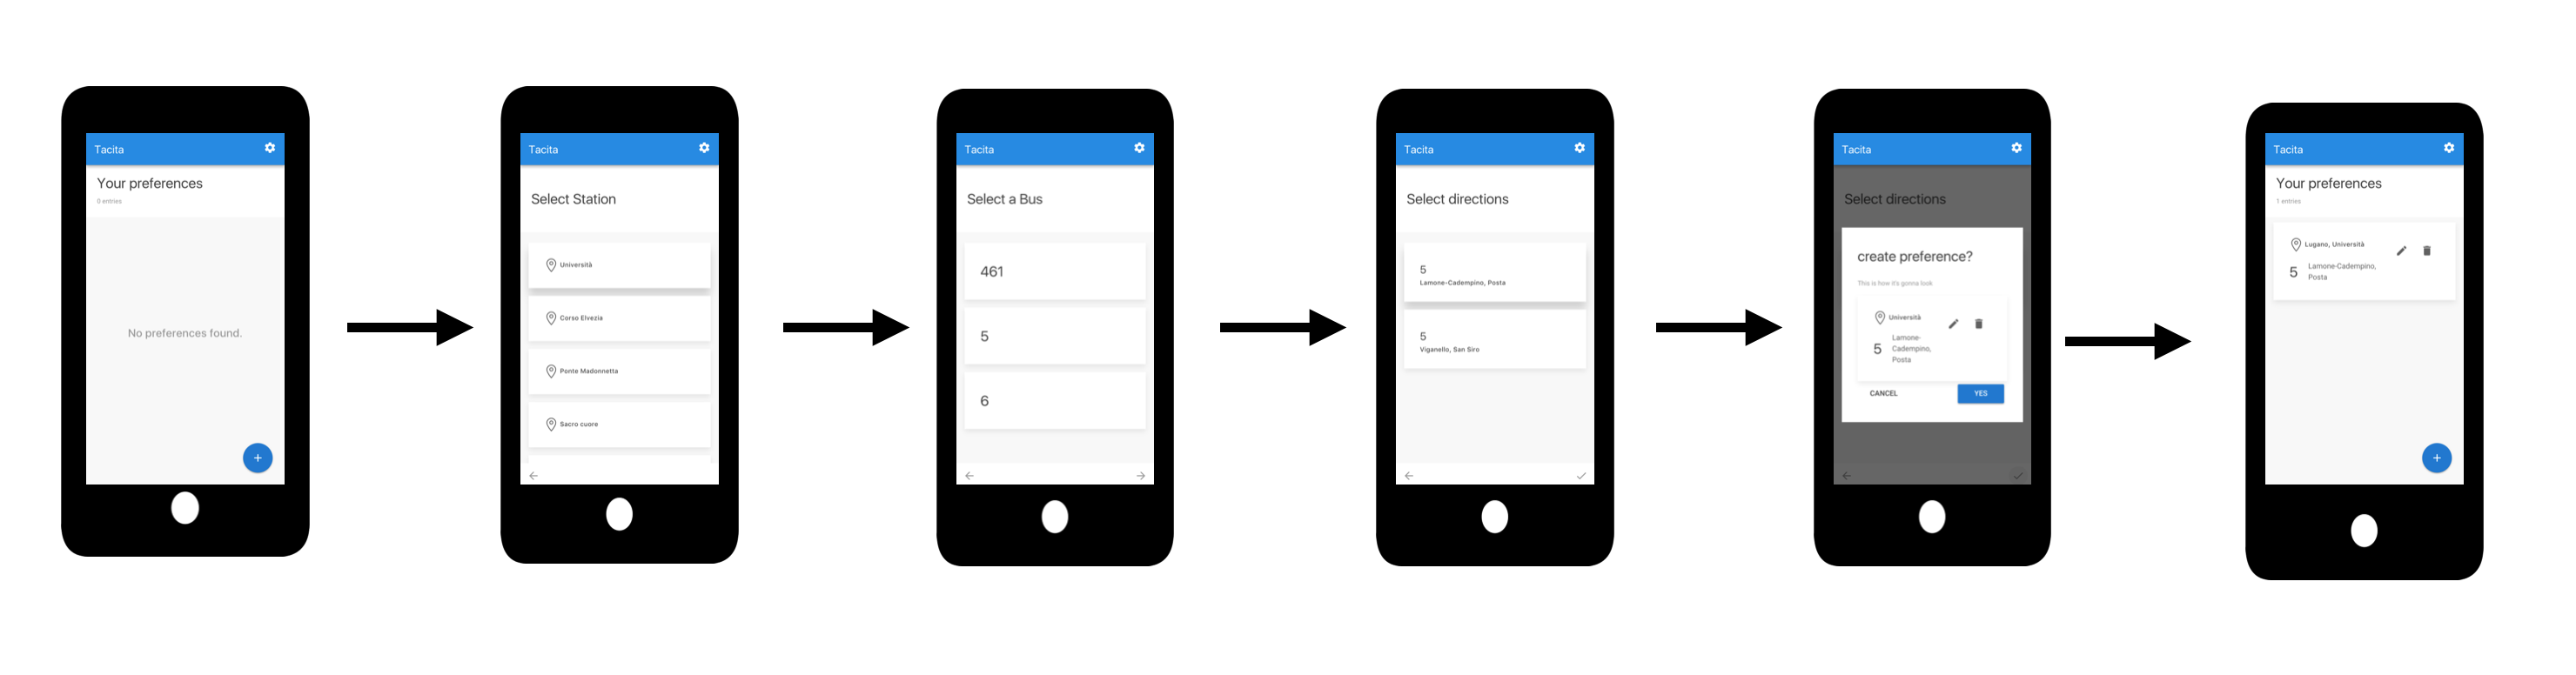
\includegraphics[width=1\textwidth]{./images/UI_flow_transport.png}
   \caption{UI flow in \emph{Transport}}

\end{figure} 


% say how ofter we clone them
% link to opendata
% put some pictures of the screen gui
% show some pictures of the preference flow
\subsubsection{Classes App}
The second application is \emph{Upcoming Classes}. It displays information about classes such as the course's schedule for the next days. It is possible to select preferences or to create queries for specific courses from the screen. All the courses are displayed on the calendar in the correct order supporting both month and week view.
Similarly to the Transport application, we had issues with the API, in our case, provided by the University itself. A single API call to know all the schedules takes more than $1500ms$ as showed in Table 1. It gets worse if you try to get all the courses for a faculty:
\begin{table}[h]
\centering
\begin{tabular}{|l|c|}
\hline
Request & Time \\\hline
http://search.usi.ch/api/courses/35255488/schedules & 1952ms \\
http://search.usi.ch/api/faculties/1/courses & 9294ms\\\hline
\end{tabular}
\caption{}
\label{table:usi_request}
\end{table}
Therefore they cannot be properly used in a real application. Even if, from the client, we always cache the request, we cannot avoid waiting for the first time. The reason why they are so slow is the response size. Their response is heavy due to a poorly model population; for each course that is sent back, tonnes of unused field are provided. Moreover, by inspecting a response for class schedules, we can notice the same huge course object appears, unnecessary, for each schedule object.
Therefore, again, we needed to clone all the API in order to just sent the right amount of information, by doing that, the previous schedule request now needs just $18$ms. Table 2 shows these results.

\begin{table}[h]
\centering
\begin{tabular}{|l|c|}
\hline
Request & Time \\\hline
http://personaal.inf.usi.ch:3000/classes/api/course/246/schedules & 18ms \\
http://personaal.inf.usi.ch:3000/classes/api/faculty/1/courses & 1000ms\\\hline
\end{tabular}
\caption[Table caption text]{}
\label{table:classes_request}
\end{table}
The display's front end application is divided into two main parts easily identifiable, the calendar and the query engine next to them. The calendar is create using \emph{fullcalendar} jQuery library that does all the dirty work of render and setting up all the events into the corrects slots. 
The courses can be selected thanks to the query engine on the right part of the screen. As soon as the user clicks on the button representing the faculty, it is guided in order to create a valid query using a step by step approach; even if it may be not the faster way, it is the safest since no wrong request can be generated. The procedure is showed in the following storyboard:
% aggiungi storyboard classi

As we did for the Transport Application, we also created a smart phone interface in order to create, remove and edit preferences. For consistency reason, we decide to keep to use the same UI design we used for the transport application.
% show transport app similar to this one
\subsubsection{Mobile Application}

A mobile application was developed in order to let users select their preferences and custom settings. In our project, each user can select a colour that is showed as a little label near the preference on the screen making it easier to identify. Since only the content owner knows is colour, anonymity is maintained in the system. The home page shows the applications list.

The user can quickly enable/disable content flow for each application by changing the state of a toggle present on each service. When an application is disabled, no information will be sent to the \emph{Map Provider}. However, since we are using socket connection, when an application is enabled the new state will be immediately broadcast to the system making screens react to it.

Each application must provide a web page to manage their specific preferences that can be access by clicking on their name in the home page of the mobile application. For instance, the \emph{Transport Application}, provides a web view to create customs preferences based on stations, buses and directions. Similarly, \emph{Upcoming Classes}, expose a web interface to manage its content. In Figure 5, the user clicked on the \emph{Transport} application revealing its main preferences page that can be see in the second frame where an already created preference is showed.

When a Bluetooth beacon is found, a floating button appears making possible to access the display page where detail information about the discovered display are showed. Automatically, users preferences will be displayed on the screen. The interactions are deeply explained into section 2.3. Figure 5 shows a usage example. From left to right, the application is opened, then the \emph{Transport} application is selected and its preference page is open. Later a new colour is picked, in our case blue. After we can observe that a display was found by clicking on the floating button that has just appeared. In the last picture, our preferences are labelled into the display with the chosen colour.
\begin{figure}[H]
  \centering
  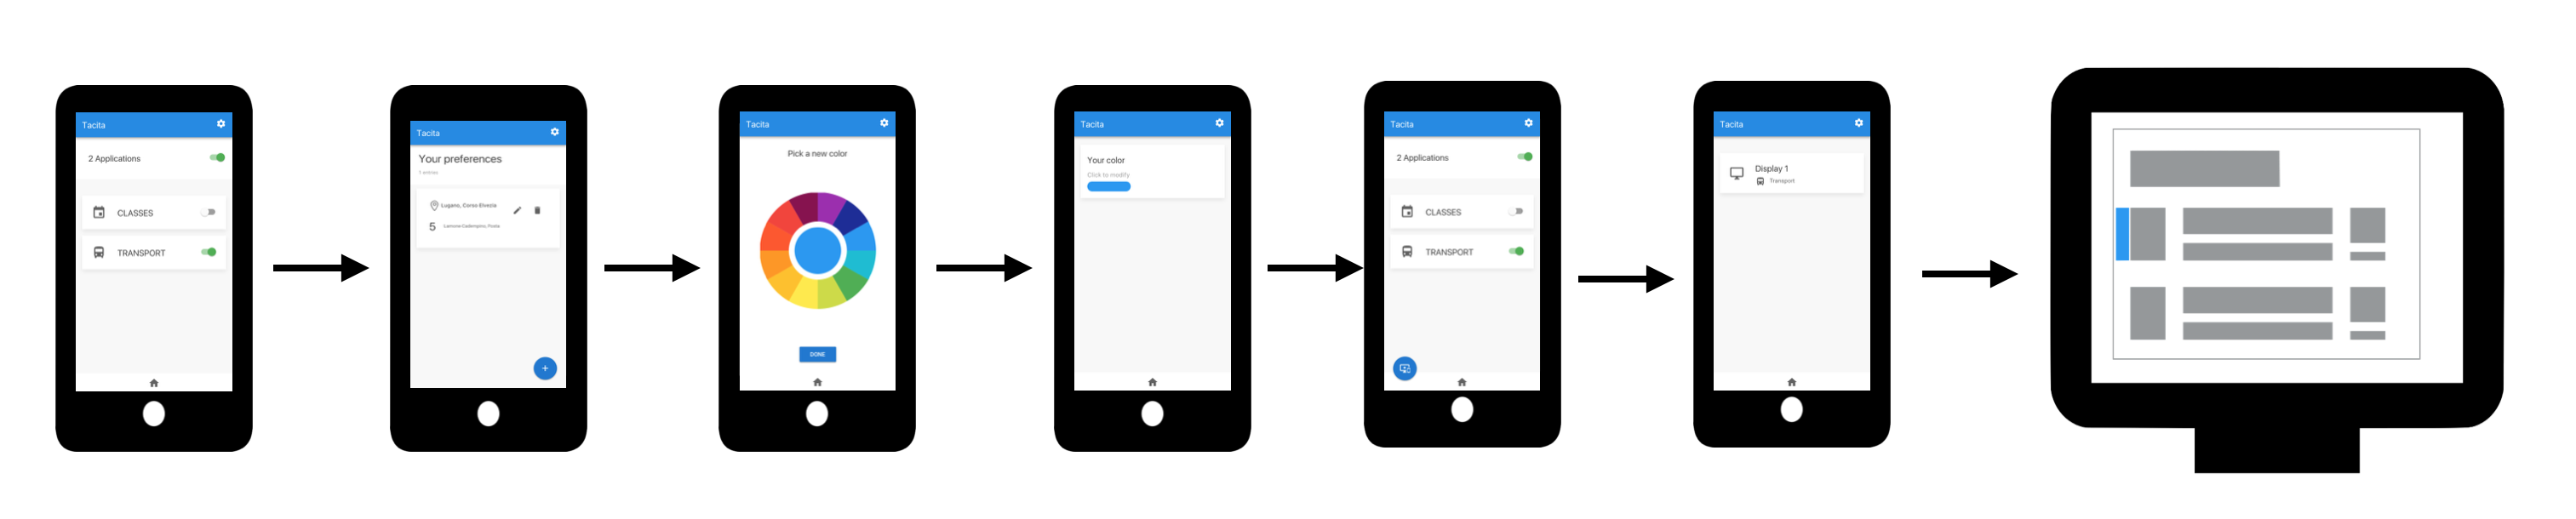
\includegraphics[width=1\textwidth]{./images/UI_flow.png}
   \caption{Mobile Application UI flow}

\end{figure}

\subsubsection{Proxy}
A simple \emph{Proxy} was created in order to proxy all the HTTP/HTTPS and web socket request. In this way, a single domain is exposed to the client so no CROS origin request is needed. Due to security reasons, sockets are only supported into the secure mode; so it is highly recommended to access our servers with a secure connection in order to experience all the features of our project
 
\subsection{Architecture Interactions}
In this section we are going to analyse all the interactions, especially between user and display, showing and explain each message that the entities exchange in order to communicate.

\subsubsection{User Client perspective}

From a User point of view, the first action that can happen is walking into a display. As soon as the mobile application detects the beacons, it gets a list of them sorted by distance (action $1.$ of Figure 6). The first one is fetched and its id is used to make a request to Map Provider ($2.$) in order to know which display is associated with it. If there is one, a message containing user's id and display's is pushed into the socket ($3.$) only if the screen application is enabled. An example message:

 \begin{lstlisting}
{
  action: 'USER_NEARBY',
  payload: {
    user_id: '1',
    display_id: '1'
  }
}
 \end{lstlisting} 
When the display receives the notification, it checks if it has the same id. If it gets the user's preference from the back-end running application ($4.$). Finally, the user's content is showed on the screen ($5.$). Similarly, when a user walks away, the connection with the beacon is lost and a new message is pushed into the socket in order to remove its preferences from the display.
 \begin{lstlisting}
{
  action: 'USER_EXITS',
  payload: {
    user_id: '1',
    display_id: '1'
  }
}
 \end{lstlisting}

To avoid processing the same information two or more times, the displays uses a in memory cache. Furthermore, a life duration is set for each of them in order to remove them if no exit event is detected.
\begin{figure}[H]
  \centering
  \includegraphics[width=0.6\textwidth]{./images/elements_interactions_user.png}
  \caption{Architecture Interactions, User point of view}
%    \subfloat[Display interactions]{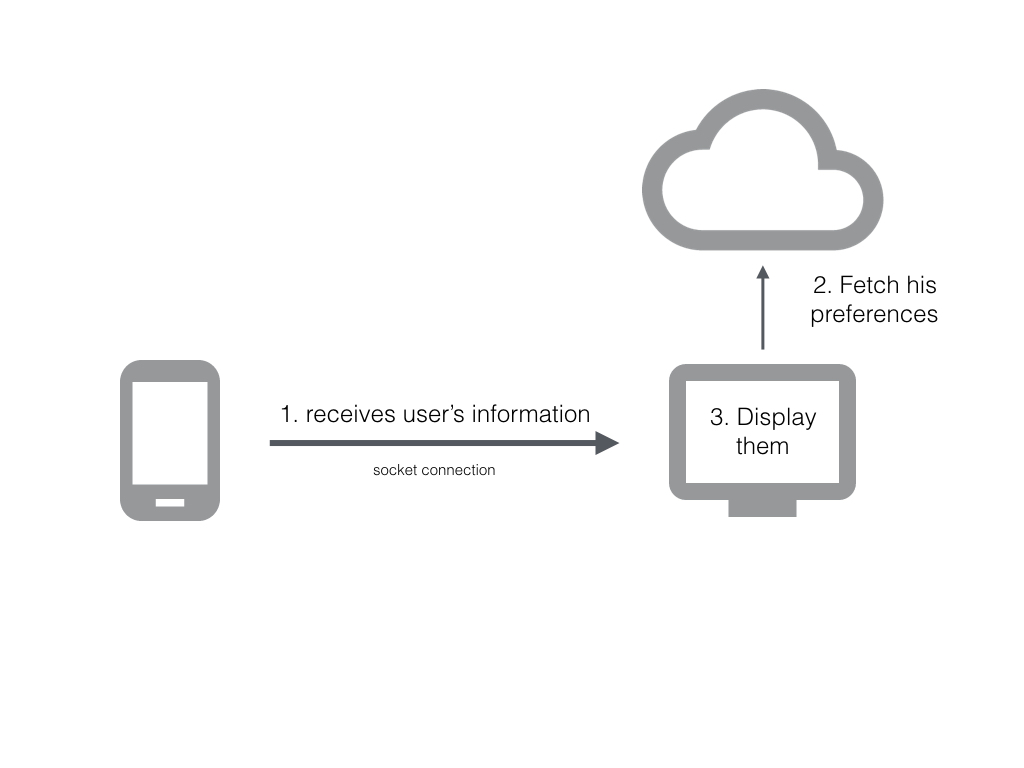
\includegraphics[width=0.5\textwidth]{./images/display_interactions.jpeg}}

\end{figure} 
\subsubsection{Display Client perspective}

When the display's web client is connected to one of the applications (action $1.$ Figure 7), it does some initial setup ($2.$). Depending on the local case, it may ask for the geo localisation, used in the \emph{Transport application} or create some data structures. After the boot phase is done, a request for the data is made to its provider in order to show information ($3.$).
In the mean time, the screen sends the its running applications id to the \emph{MAP Provider} ($5.$) in order to update its state. Then the \emph{Provider} broadcasts to all the clients the new information using sockets so each element has a global real-time view of all the displays state. In our project, the mobile application, when it receives such information and if the new application running is enabled, it sends again the user's identifier in order to show the personalised content into the new application without reloading the view.
\begin{figure}[H]
  \centering
  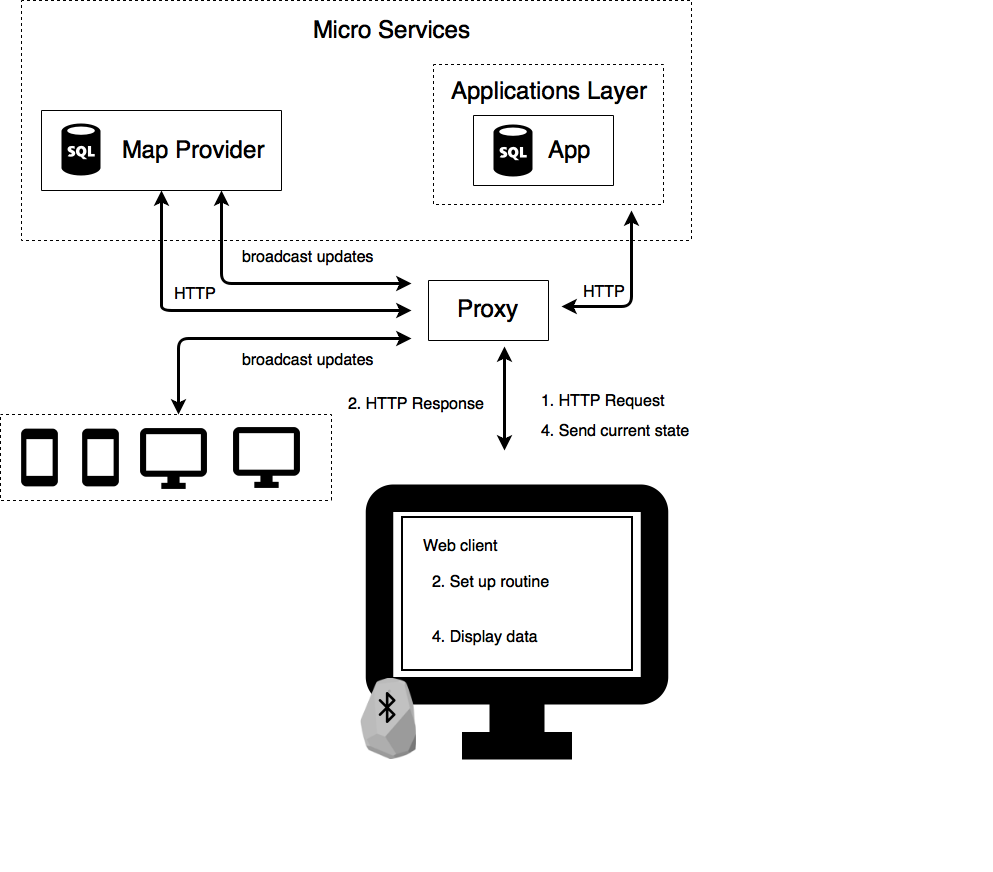
\includegraphics[width=0.6\textwidth]{./images/elements_interactions_display.png}
  \caption{Architecture Interactions, Display point of view}
%    \subfloat[Display interactions]{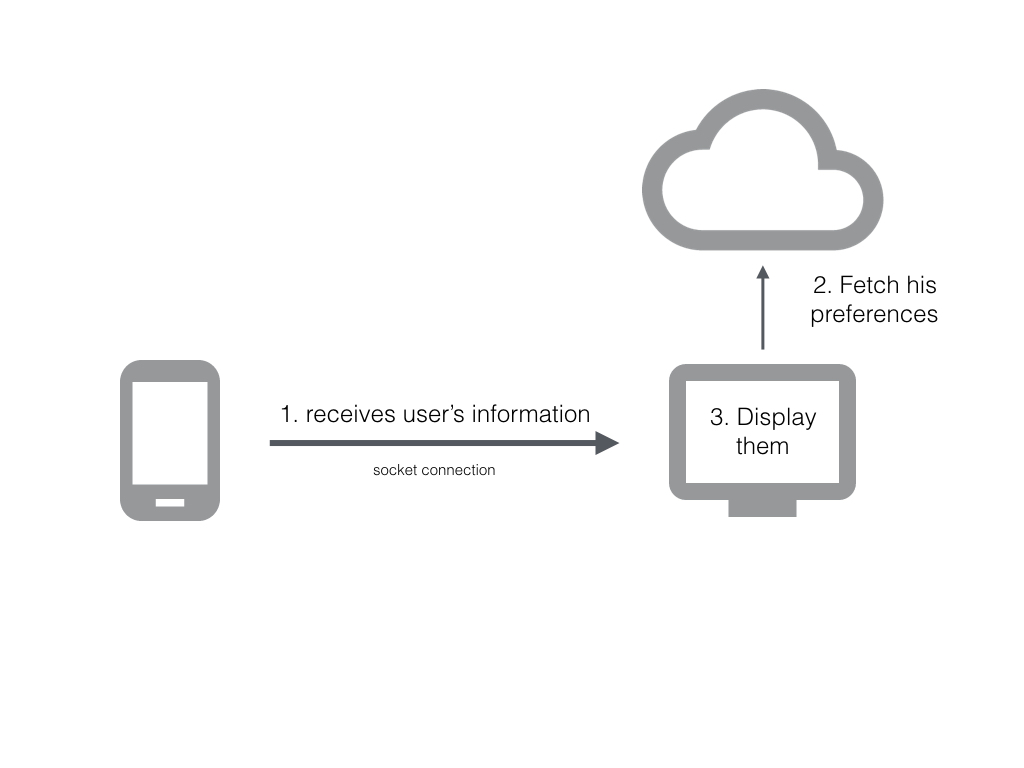
\includegraphics[width=0.5\textwidth]{./images/display_interactions.jpeg}}
\end{figure} 
At each screen is associated a unique id. Therefore, before deploying a display, it must create a new entity in our database by making the correct request to the \emph{Map Provider}. The id is passed to the display's client by adding it in the end of the URL that is processed by the front-end software.
\subsection{Architecture Technologies}
In this section we introduce each technologies used for both the back-end and the front-end. For this project, we chose the latest technologies and programming languages in order to provide a service that will last for a long time without being obsolete. The display used in this project is a \emph{iiyama} prolite th4664mis with an Intel NCU running Windows 10 and \emph{Google Chrome} as web browser.


%\subsubsection{Display Client}
%The display used in this project is a \emph{iiyama} prolite th4664mis with an Intel NCU running Windows 10 and \emph{Google Chrome} as web browser.
% but our architecture can support any operating system and all the major, since it only needs a web client to run it. Since the applications are \emph{interactive} it is possible for the audience to interact with them using a touch interface to click on the applications' pages discovering new content.
%
%Bluetooth beacons are physically placed nearby to make them visible from the mobile application and create walk-by contact personalisation. They are placed into key points of the university, such as, \emph{mensa} or at the entrance of the faculty. It is very important to accurately study where to place them to maximise the number of viewers. Users can temporally control them by creating preferences that are showed when they walk-by. Furthermore, the running application can be dynamically changed by making a REST call to the \emph{Map Provider} that will notify the screen through sockets and make it updates its state.

\subsubsection{Back-End}
We firstly started to develop the first application using Django, a widely used Python web framework, but we encounter some issues with web socket that were not supported "out of the box".
So, we decide to completely switch both language and framework by choosing Swift 3 and Vapor.
Swift is a "powerful and intuitive" open source programming language developed by Apple in 2015 for both MacOS X and Linux. It is a Protocol Oriented Programming Languages.
%\\
%\emph{A protocol defines a blueprint of methods, properties . The protocol can then be adopted by a class, structure, or enumeration - Apple}
Unlike classes, the fundamental of Protocol Oriented Programming, POP, is Value Type encouraging flat and not nested code. This benefit is reflected in its performance and flexibility.
The syntax is concise yet expressive, it uses labels and spaces to improve the code readability making possible to write complete sentences only with code. Apple wanted to create a product that was at the same time, feast and beauty.

After selecting a programming language, we need a framework to create our applications. We chose Vapor, a powerful, beautiful and easy to use MVC framework to build web servers. We developed all the web servers we used in this work with this framework.
Vapor is easy to start with thanks to the clear APIs that, not also speed up the developer work, but make the code more maintainable and more understandable. One of his strength points is the performance inherited from Swift.
Vapor uses a Model View Controller design pattern that divides an application into three decoupled interconnected parts in order to separate internal representations of information. A \emph{Model} directly manages the data and logic about a database entry such as display or beacon. The \emph{View} outputs a representation of an information, in our case, the web page. The third part, the \emph{Controller} acts on both \emph{View} and \emph{Model}. It controls the data flow into the model, updating its state, and change the view whenever is needed.
\subsubsection{Front-end}
In order to archive the best results in term of scalability and performance we used Vue.js as main front-end framework. Vue.js is a library for building interactive web interfaces, it uses web components to provide a convenient way to organise an application by decoupled its element into blocks.
A web component is similar to an Object Oriented programming classes, it encapsulates all the logic behind a certain functionality of the application. In Vue, a component, is formed by three parts: \emph{template}, \emph{script} and \emph{style}.

The \emph{template} allows the developer to write HTML and to include variables, conditions and loops. Moreover, thanks to built-in loaders, it is possible to easily use any pre-processing HTML library such as Pug. 
The second part, the \emph{script}, is the core of each component. As the name may suggest, it is the code part. Each component exposes a Javascript object allowing Vue to grab it and render it in the proper way.
The last tag, \emph{style} is were is possible to custom style a component using CSS or css-processors such as  Less or Sass.
One of the main advantages of Vue over other front-end framework is \emph{reactivity}. Reactive programming is a synchronous programming paradigm concerned with data streams and the propagation of change. It uses Observers in order to trigger events every time a change of state is detected; therefore Vue can automatically call a render only in the part that was actually mutated minimising the DOM access and increasing speed.
A deep comparison with other frameworks can be fount at: https://vuejs.org/v2/guide/comparison.html.

Each component represent a feature, a part of the web application; it may happen that one of them need to communicate with another, maybe after a change of state or a user event. In order manage the data flow we used the Flux pattern. The main idea behind this pattern is that the state can be mutated thought actions that are reduced into the stores. Flux is composed of four parts: \emph{Dispatcher}, \emph{Store}, \emph{Actions} and \emph{View}. Their interactions are showed in Figure 8.
The \emph{Dispatcher} is a singleton that receives \emph{Actions} and dispatches them to every store that has registered with it. Each \emph{Store} receives each \emph{Action}.
The \emph{Store} is only source of truth in the applications; it holds its state and manages the logic behind it. The data must only be mutated by responding to and action by emitting a "change" event.
\emph{Actions} are the internal API of each application, they define all the possible interaction that may happen. They are plain javascript object composed of a type field and some data.
\emph{Views} displays store's data; in our application, a single view is a Vue component.

We developed our Flux library from scratch, called \emph{Flue}. Our library aims to provide a better object oriented approach than the existing one. You can find examples and documentation at our Github repository: https://github.com/FrancescoSaverioZuppichini/Flue.

\begin{figure}[H]
  \centering
  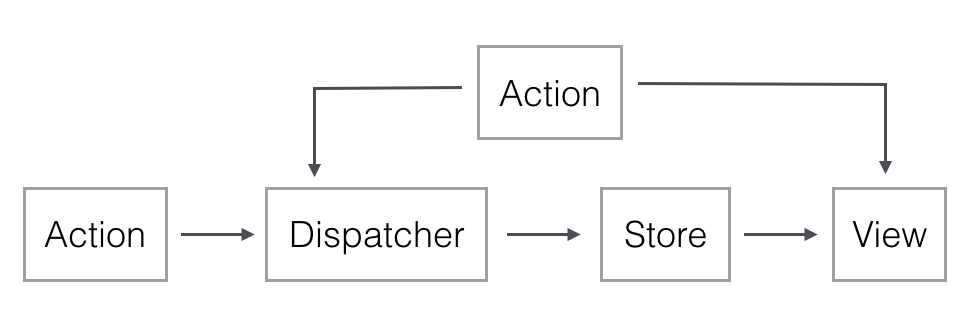
\includegraphics[width=0.5\textwidth]{./images/flux_data_flow.png}
  \caption{Flux data flow}
\end{figure} 
\subsection{Architecture Scalability}
Scalability is the ability of a system to grow larger with minimum changes. In the previous sections we often talk about how some design choices lead to an improvement in term of scalability, such as adopting a \emph{micro services} approach. In our specific case, our system state can change very quickly at any moment due to external decisions, for example if the provided buy new displays or new applications are available.
In order to make it possible to deploy independently from the network a new application, we abstract the its concept creating a layer of services that can be expanded very easily. The developers can create a new applications by just creating a web server being conform to our generic interface and expose his url.
Another possible problem that may appear is when a display is moved away. We explained before how each screen running \emph{Transport}, when its connected, fetches its position and uses it in order to communicate with Google Maps API to show real direction indications. If such problem appears, very easily, the provider just need to refresh the screen and the front-end software will automatically update itself.
Also displays can be removed or added by simply using \emph{Map Provider} REST API. Imagine screen breaks, then the associated beacon can be moved to another screen or the display may be replaced. The last case is the simplest, since we can just turn on the screen and use the last display's id, if no new device is available then the beacons can be quickly be linked to the a new screen.
\section{Design Interface}
Our application is exposed to a heterogeneous audience, therefore a clear and effective interface is mandatory to ensure a global usability. 
We have also to provide a no blocking content flow in the displays' applications, meaning that an interaction should not prevent, or block, another.
Moreover all the state changing must be displayed using design techniques, such as well targeted animation, in order to make the user understanding what is happening around him.
We decided to follow a \emph{content first} strategy by making the content clear and visible using a minimalistic approach; no unused element is present in any application. We chose cards as an only way to organise information. A card is a sheet of material that serves as an entry point to more detailed information proving a convenient way to display content composed of different elements.
% qualche efoto di card
\subsubsection{Display Applications}
The main challenge was to design for a big touch interface. We started by keeping in mind that every information must be quickly reachable and accessible; the user must understand in a fraction of second what he needs. By keeping that constrains in mind.
Our design process starts with wireframes; representing the skeleton of the application exposing its main functionalities. They are terribly useful to get a first general look of what the application is going to be. For what concerns the Transport service, we began by discarding every not necessary element following, as we said, a minimalistic approach. In the following picture, you can see the first wireframe's muck up and the final product
\begin{figure}[H]
  \centering
  \subfloat[wireframe]{\includegraphics[width=0.48\textwidth]{./images/transport_wireframe.png}}
  \hfill
  \subfloat[final product]{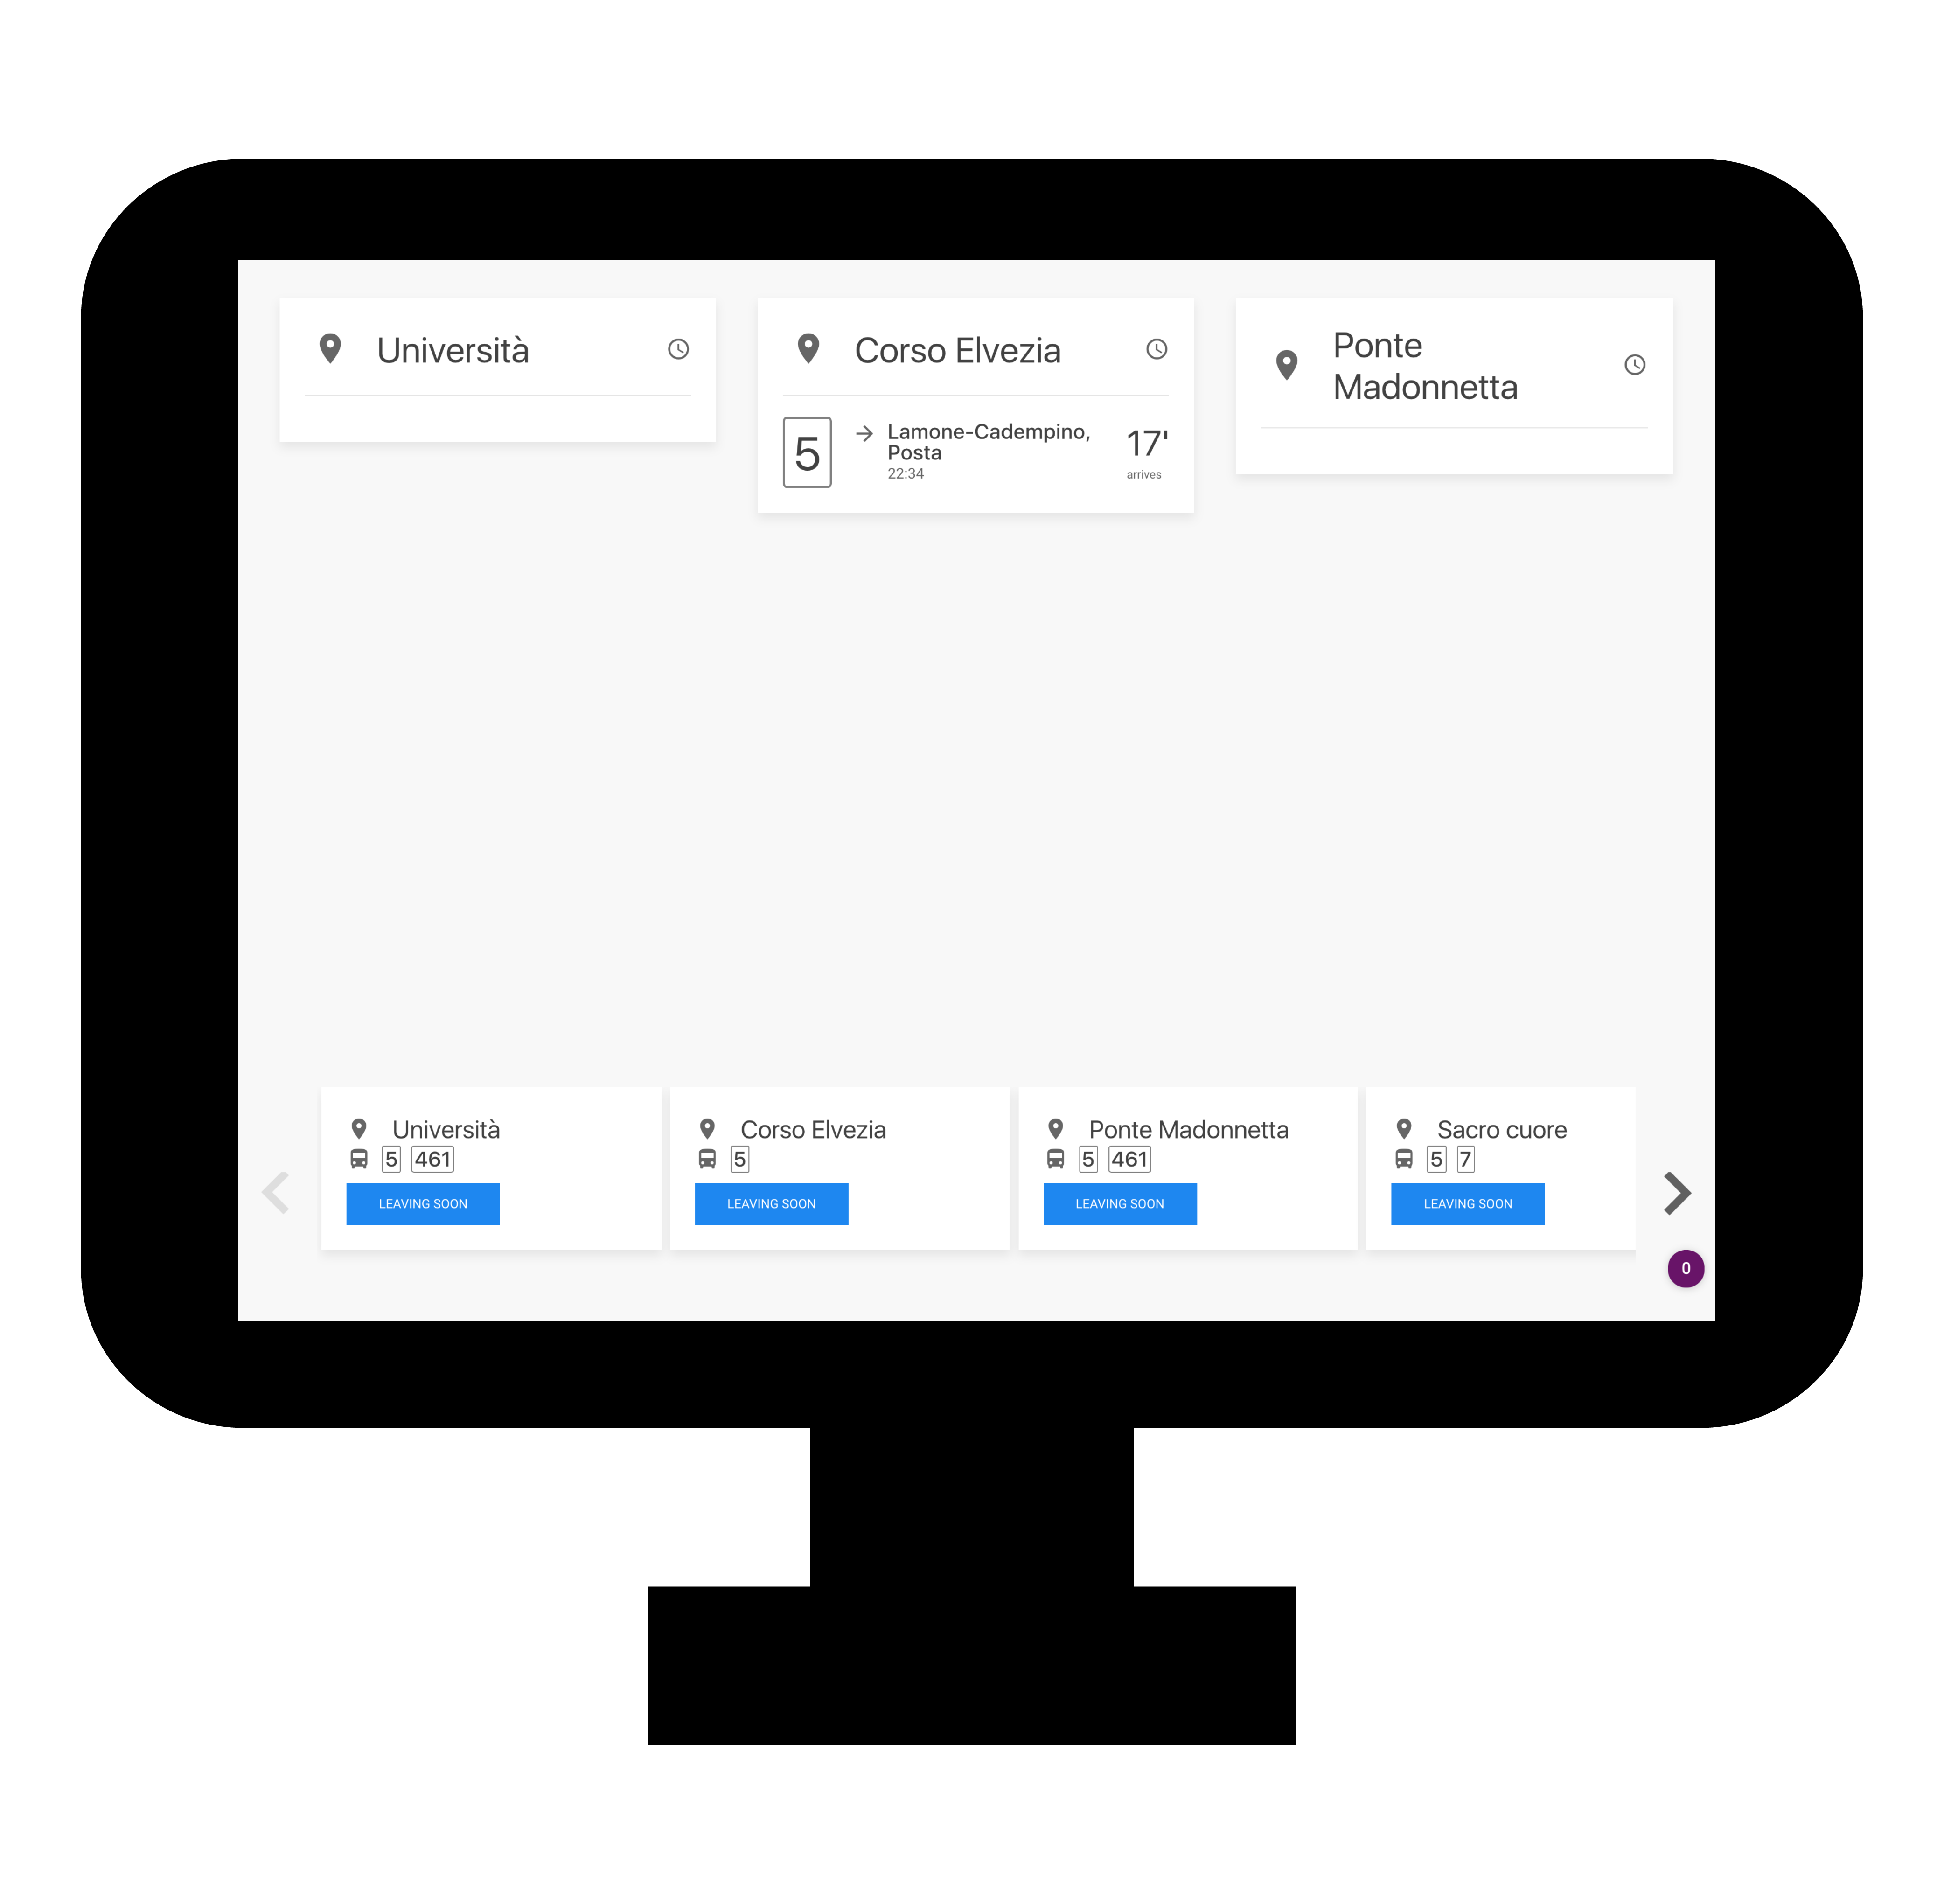
\includegraphics[width=0.5\textwidth]{./images/transport_application.png}}
  \caption{Transport Application}
\end{figure} 
If you look at the left image you can notice that all the functionalities are intuitively recognisable. In our design, studied to be used in public displays, we focused on the interactive part. At the bottom of the application there is a carousel used to change the station on the fly. Two huge arrows allow viewers to easily select mores stations by clicking on them. Moreover, all buttons are big enough to be easily touched from everyone without any problems.
We used animation to increase the user experience. For example, when a station is selected, it is pushed on the right part using a slide-in in animation making more visible. Furthermore, an open station shakes when a user tries to re-open it, giving a strong visible feedback of where it is on the display. 

In the Class application we used the same approach, we started by sketching the wireframes and defining the main functionalities. In this specific case, we needed two components: a Calendar and a query engine to search courses. 
\begin{figure}[H]
  \centering
  \subfloat[wireframe]{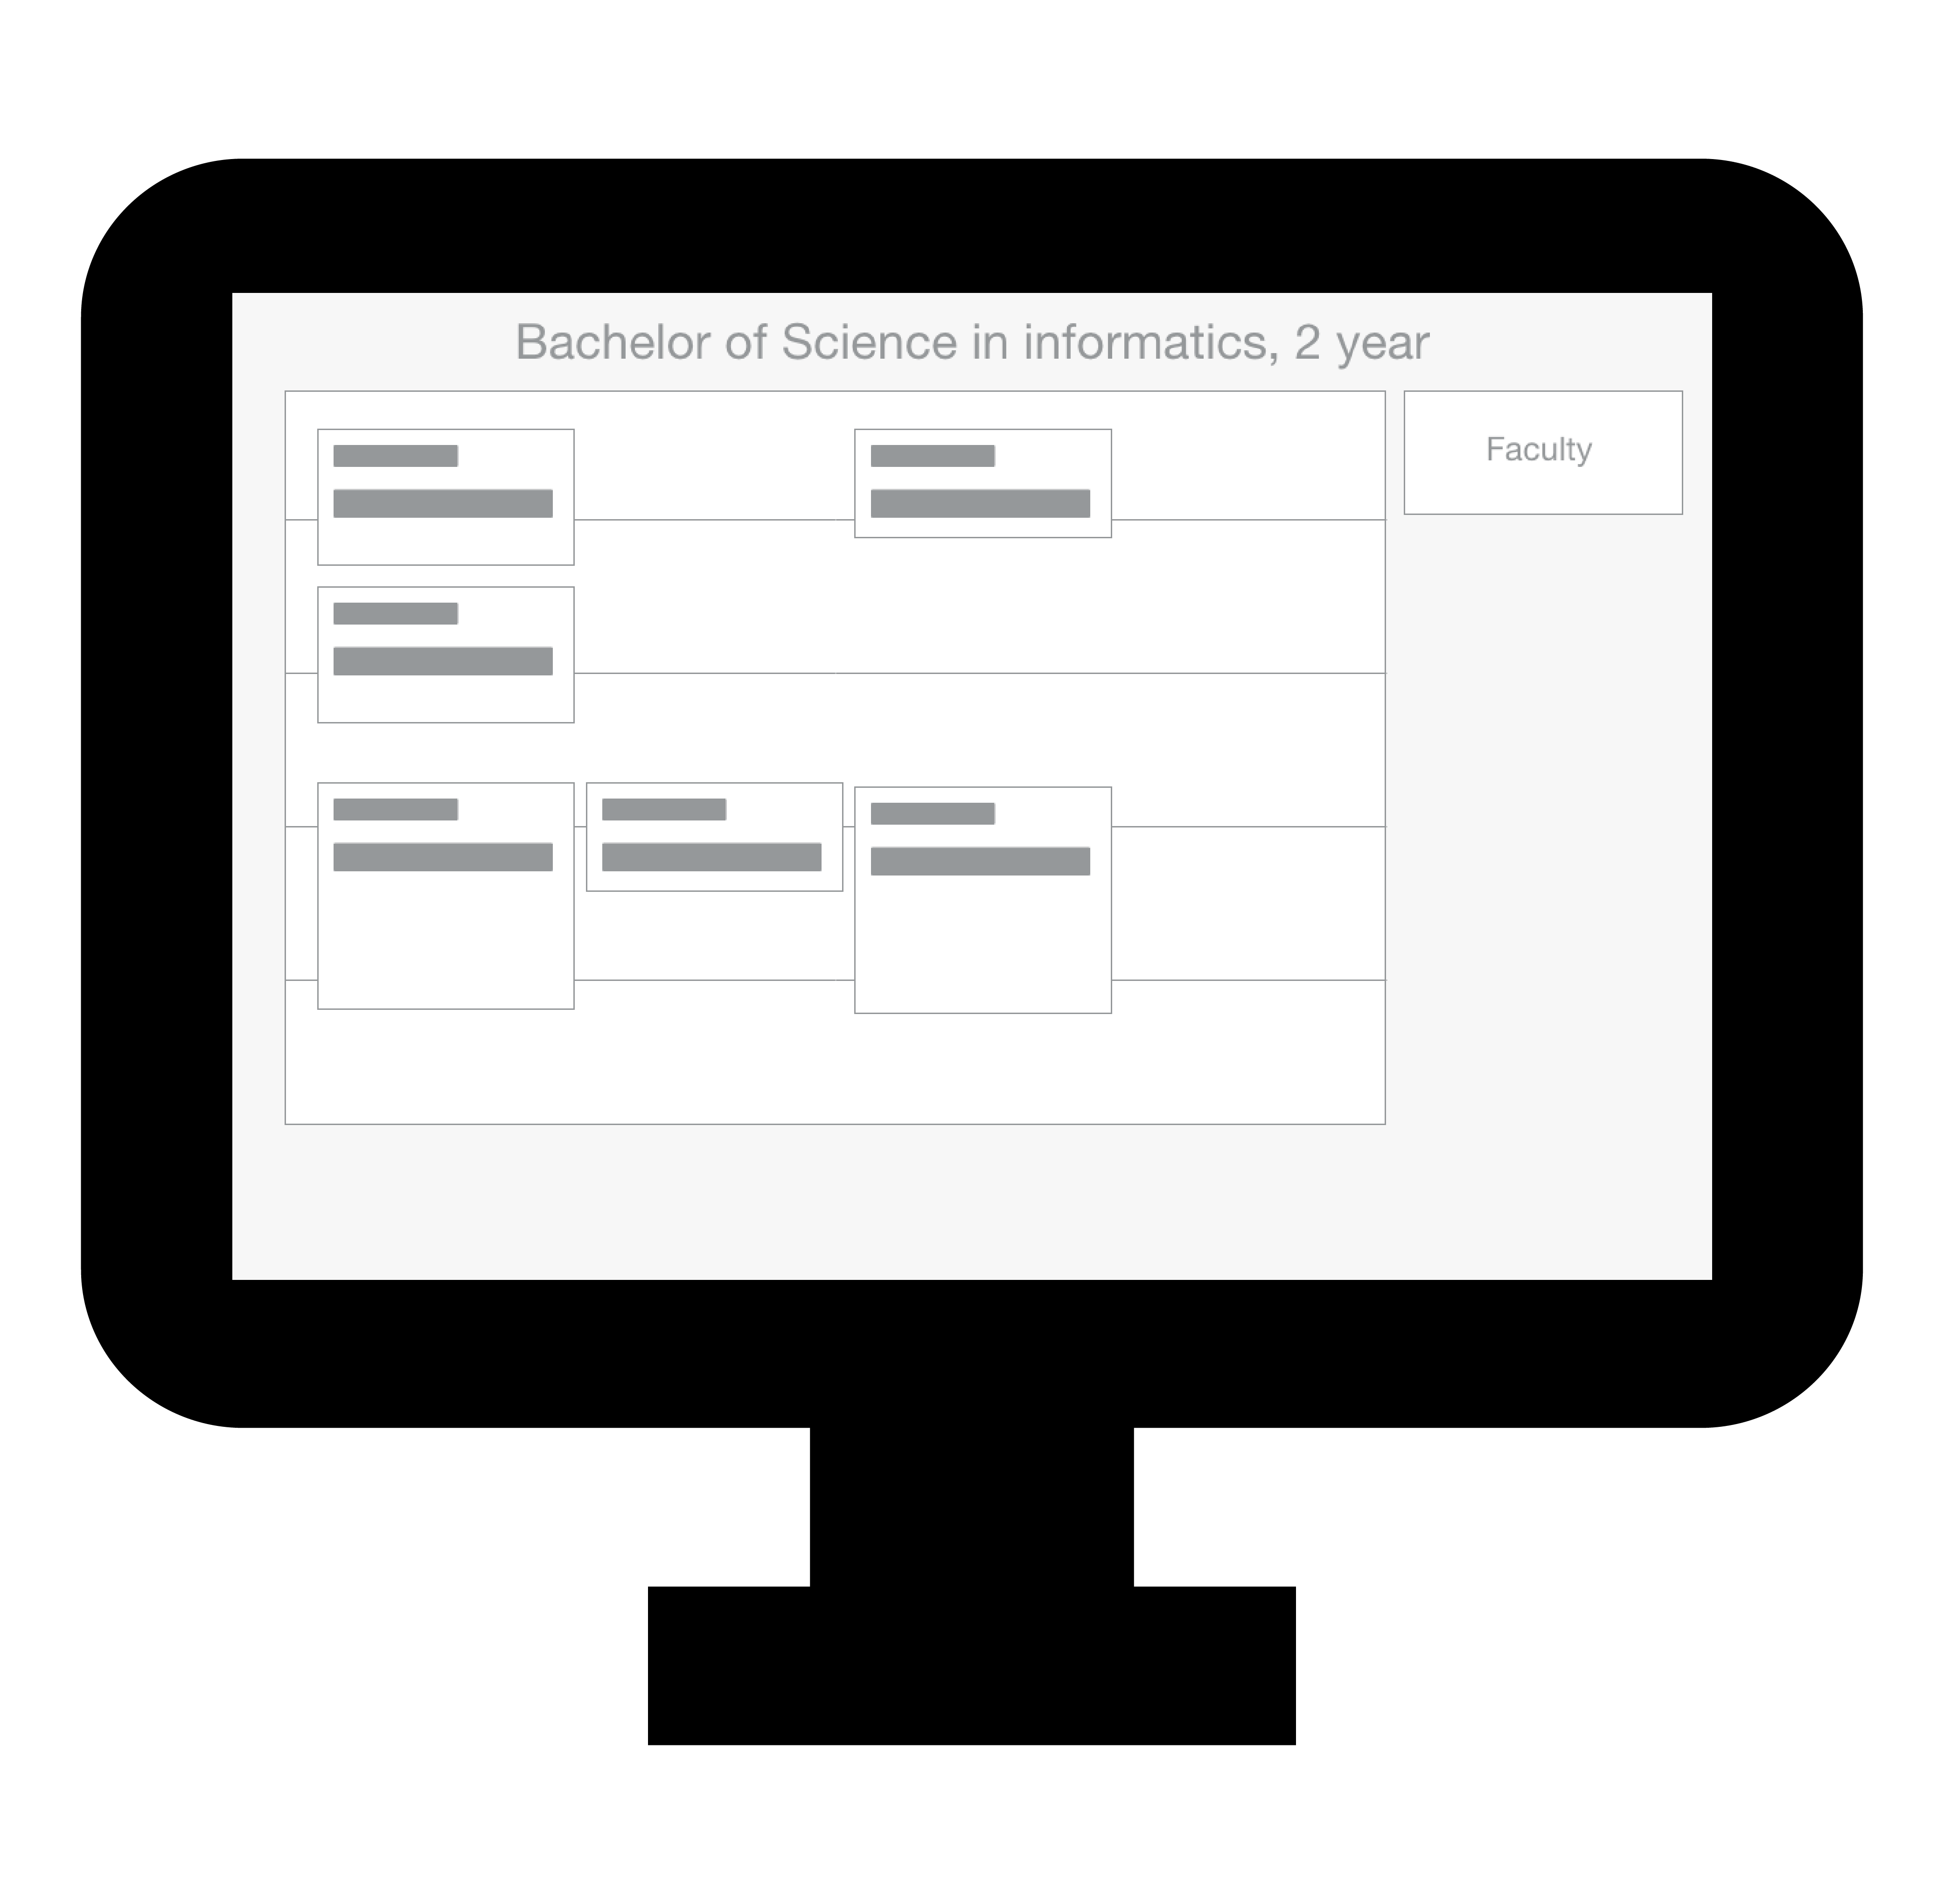
\includegraphics[width=0.5\textwidth]{./images/classes_wireframe.png}}
  \hfill
  \subfloat[final product]{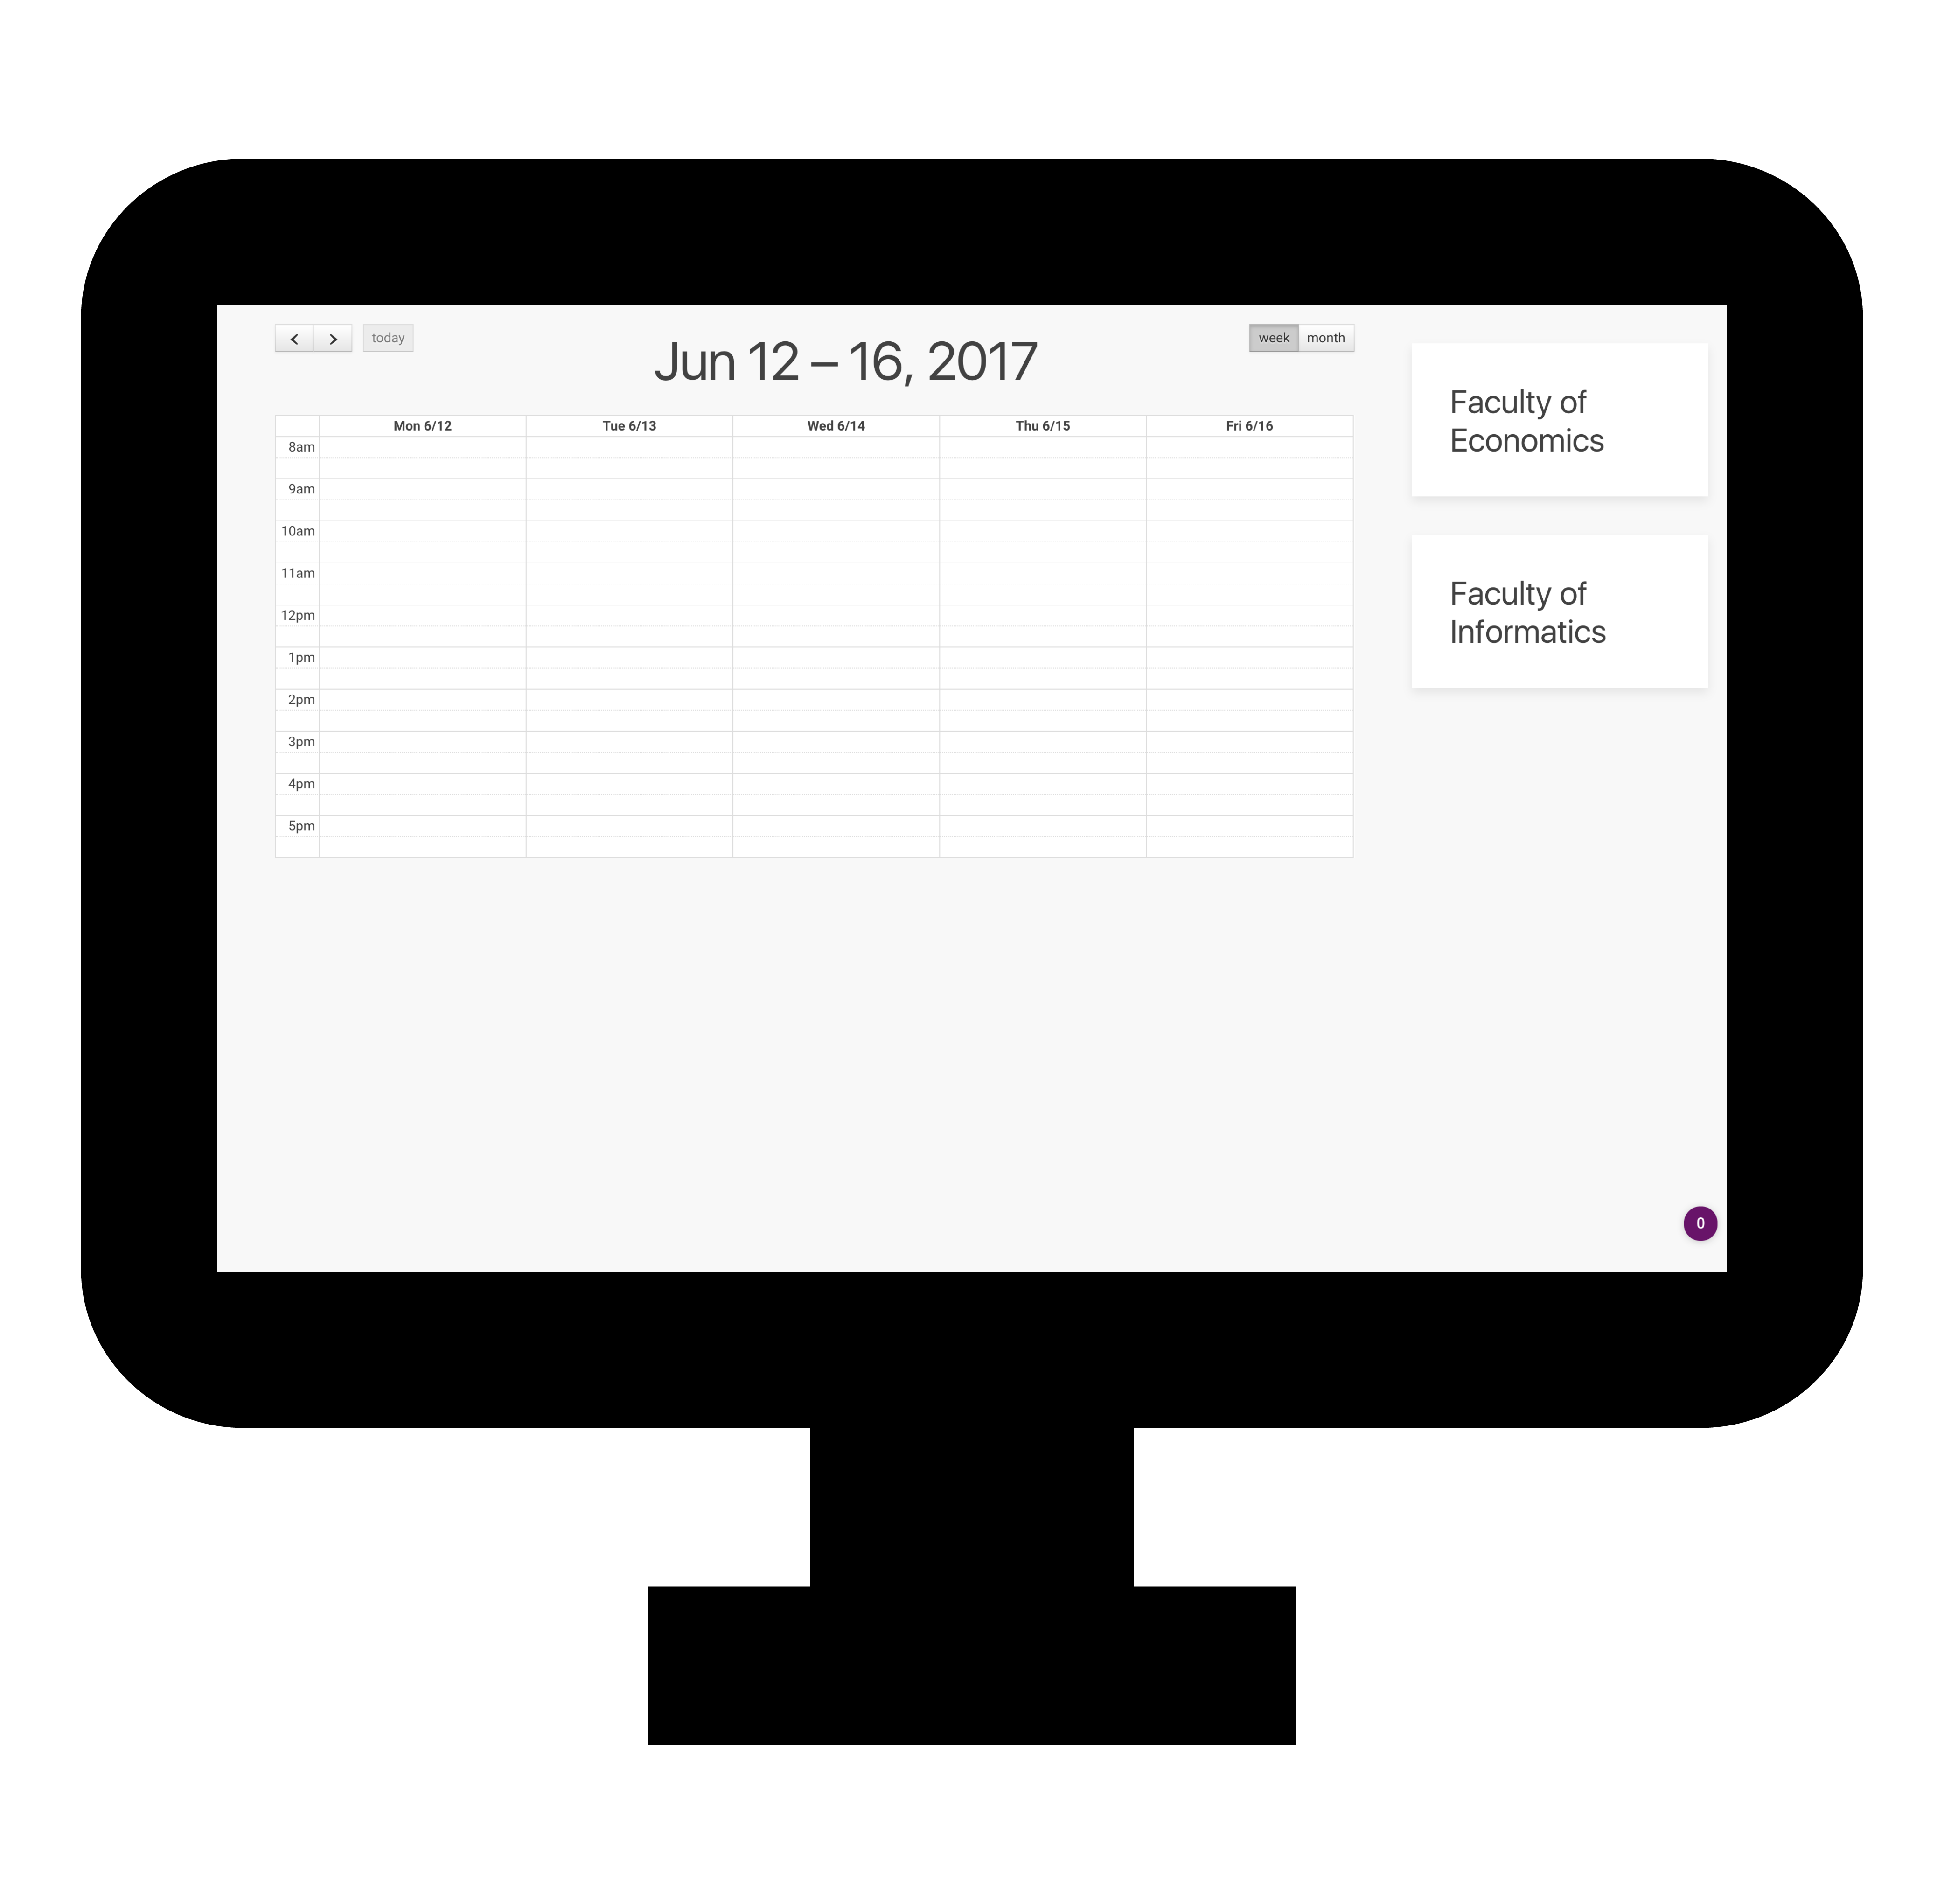
\includegraphics[width=0.5\textwidth]{./images/classes_application}}
    \caption{Classes Application}
\end{figure}
\subsubsection{Smartphone}
We develop a \emph{mobile application} to organise the user preferences, chose customisable settings and manage interactive applications. We design it from sketch to be accessible for everyone from everywhere. In main page of the application is possible to see a card list of all the existing application exposed by the \emph{Application layer}. From each application's card is possible to use a toggle button to enable or disable it. Skeletron loaders were chosen instead of classic spinner to create a more comfortable user experience. Therefore, in case of slow internet, is possible to guess the content of a page. Figure 11 shows this strategy. As you may notice, it is easy to understand how the content is going to appear on the application. We took advantages of such design pattern in almost all of our applications.
%\begin{figure}[H]
%\centering
%\subfloat[Loading]{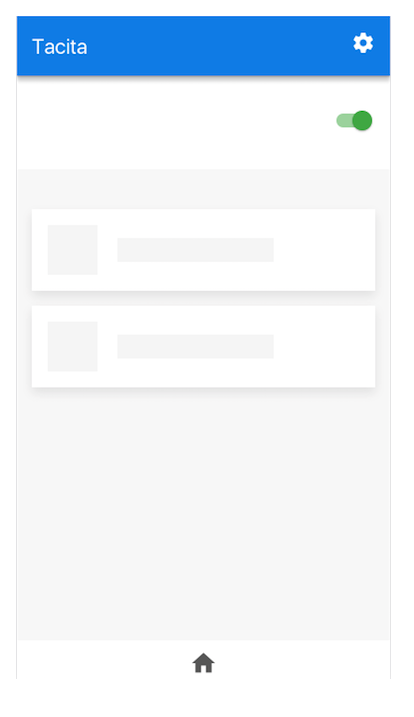
\includegraphics[width=0.4\textwidth]{./images/tacita_skeletron}}
% \subfloat[Finish]{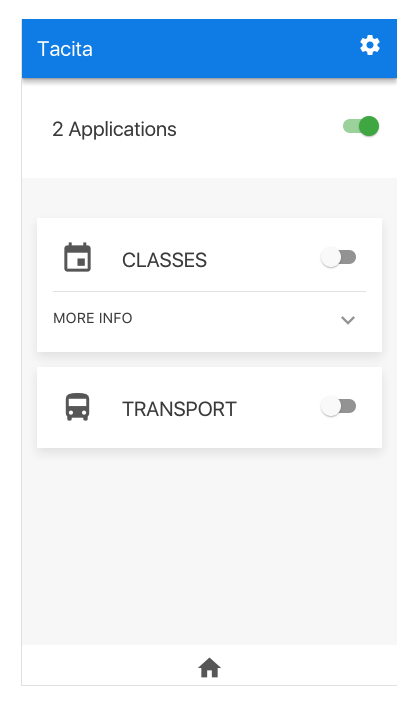
\includegraphics[width=0.4\textwidth]{./images/tacita_main}}
%\caption{Skeletron loading}
%\end{figure}
\begin{figure}[H]
\centering
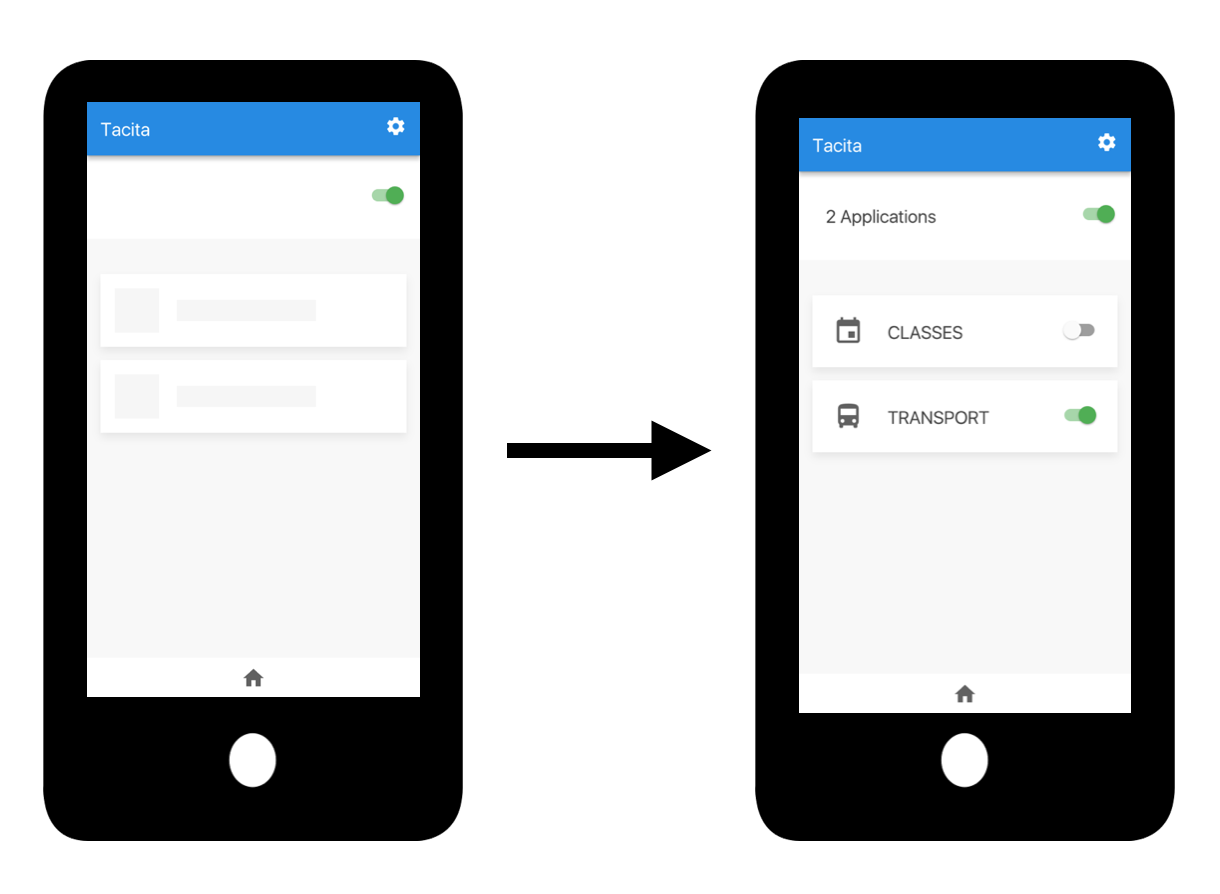
\includegraphics[width=0.5\textwidth]{./images/smartphone_loading_applications}
\caption{Smartphone home page}
\end{figure}
For each application, a toggle button is present on the right of the container to enable and disable it. Moreover, a global toggle button is available on the top of the page allowing to enable of disable all the applications in one click. In the case that a provider adds a description for an application, then it is possible to read it using the arrow at the bottom of each card.
In figure 13 is present the UI flow that occurs when a User walk nearby a screen. A floating button pops up making the displays page available. These buttons represent a great way to quickly add a functionality to a view, we decided to create a pulse animation to increase its visibility in the page. Display page shows all the discovered displays from the detected beacon and, since, we are using socket connection, if the display changes the running application, the client will be notified updating its view.
\begin{figure}[H]
\centering
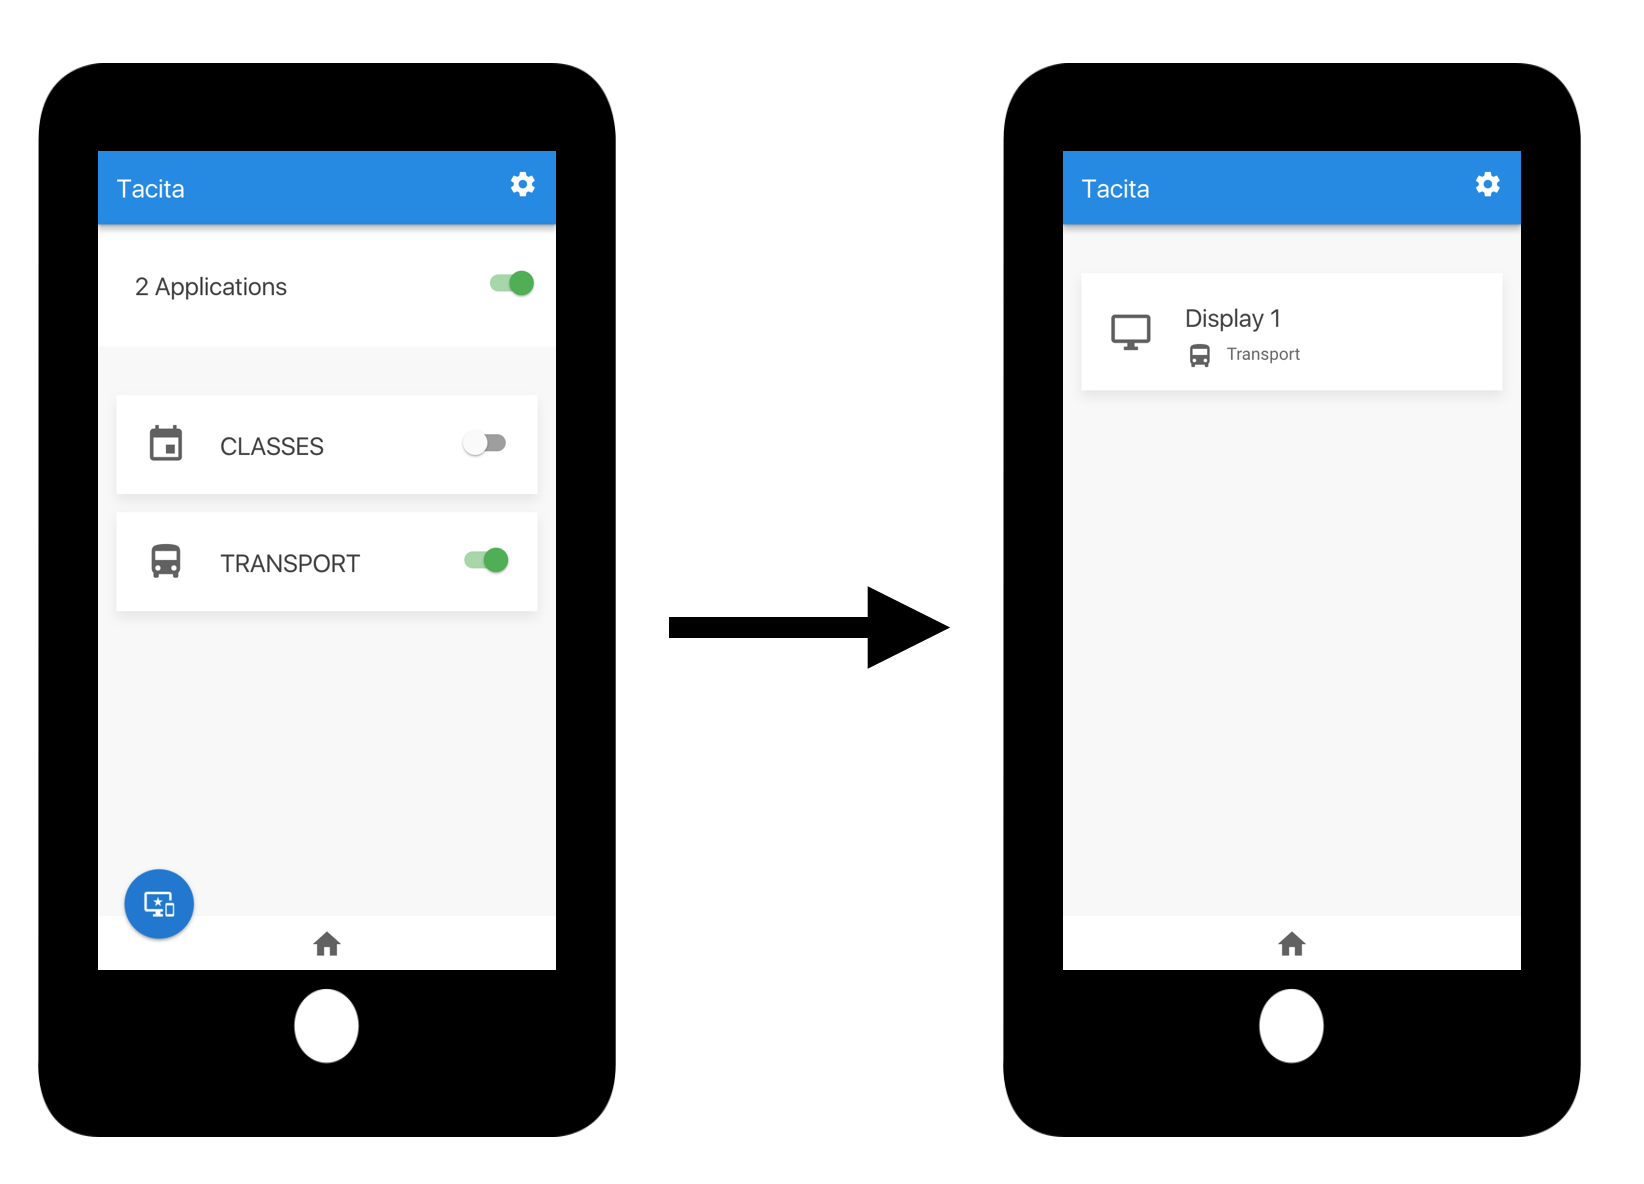
\includegraphics[width=0.5\textwidth]{./images/smartphone_displays}
\caption{Display found}
\end{figure}
As we said before, we  provide a convenient way to select a custom personalisation. We chose a colour based approach in order to highlight the visibility of an own content. The user can pick up a colour from the wheel and use it to find his preferences on the screens. Moreover, our system can easily support any other identifier such as username or avatar.
\begin{figure}[H]
  \centering
  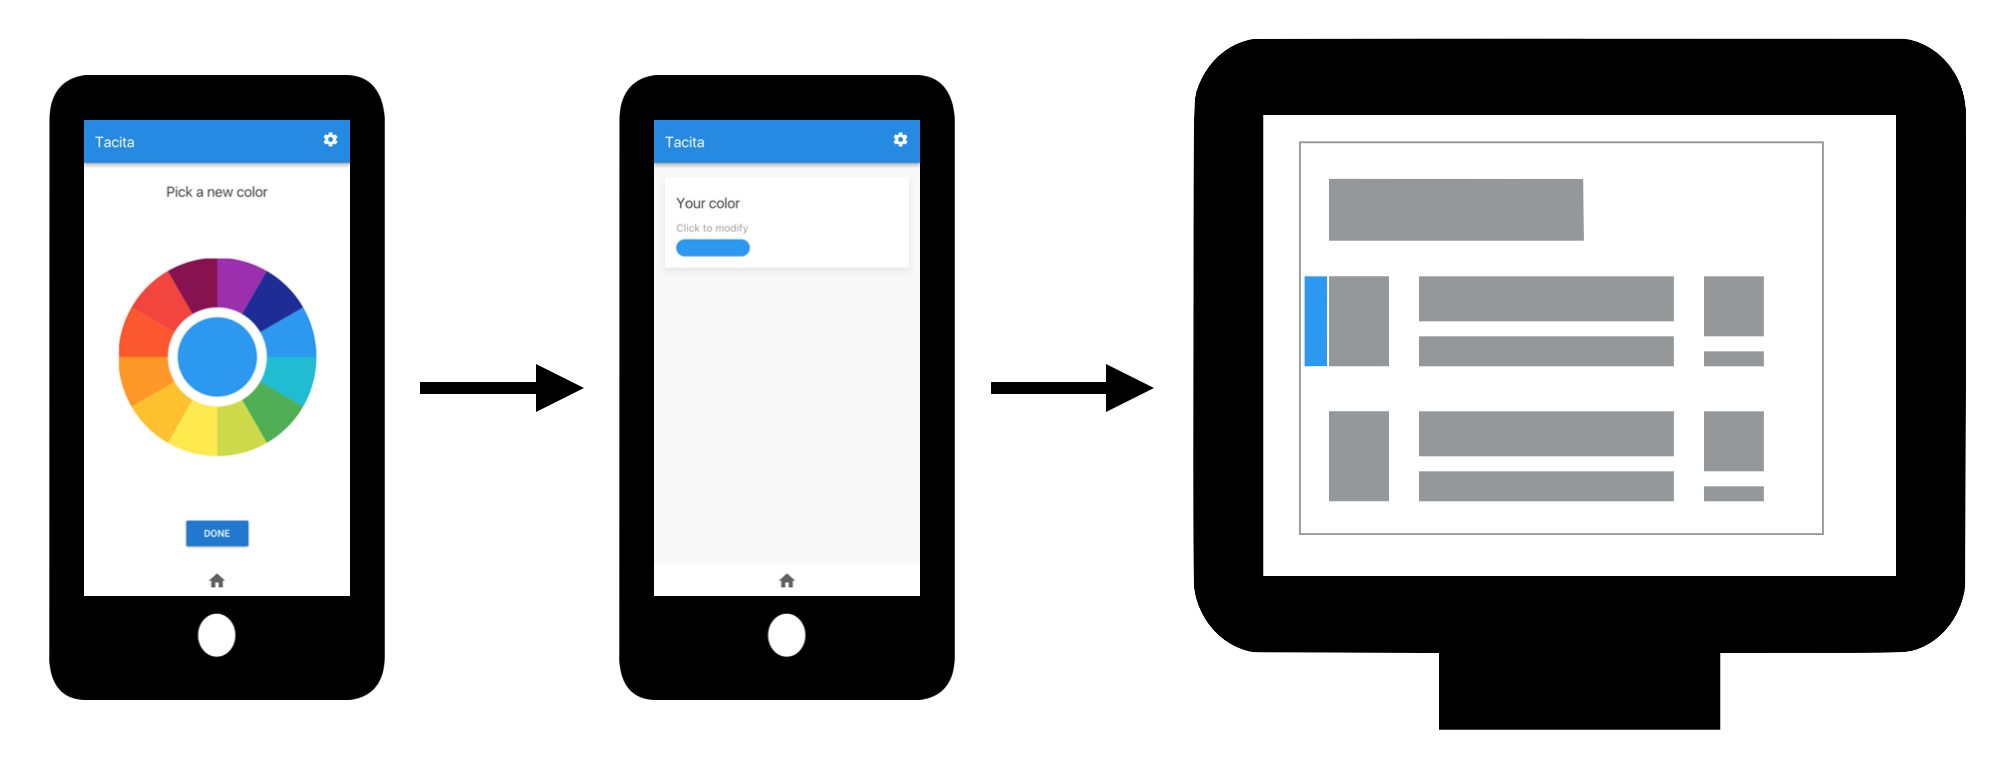
\includegraphics[width=0.7\textwidth]{./images/smartphone_color_preference}
  \caption{Preference on display}
\end{figure}
In Figure 13, an user selects a "blue" colour as preferences' identifier by clicking on the colour wheel and press "done". Then, when a screen displays the personal content, a little label is added on the left part of preferences. If one of more users walk in, then the label is split as it is showed in Figure 14.
\begin{figure}[H]
  \centering
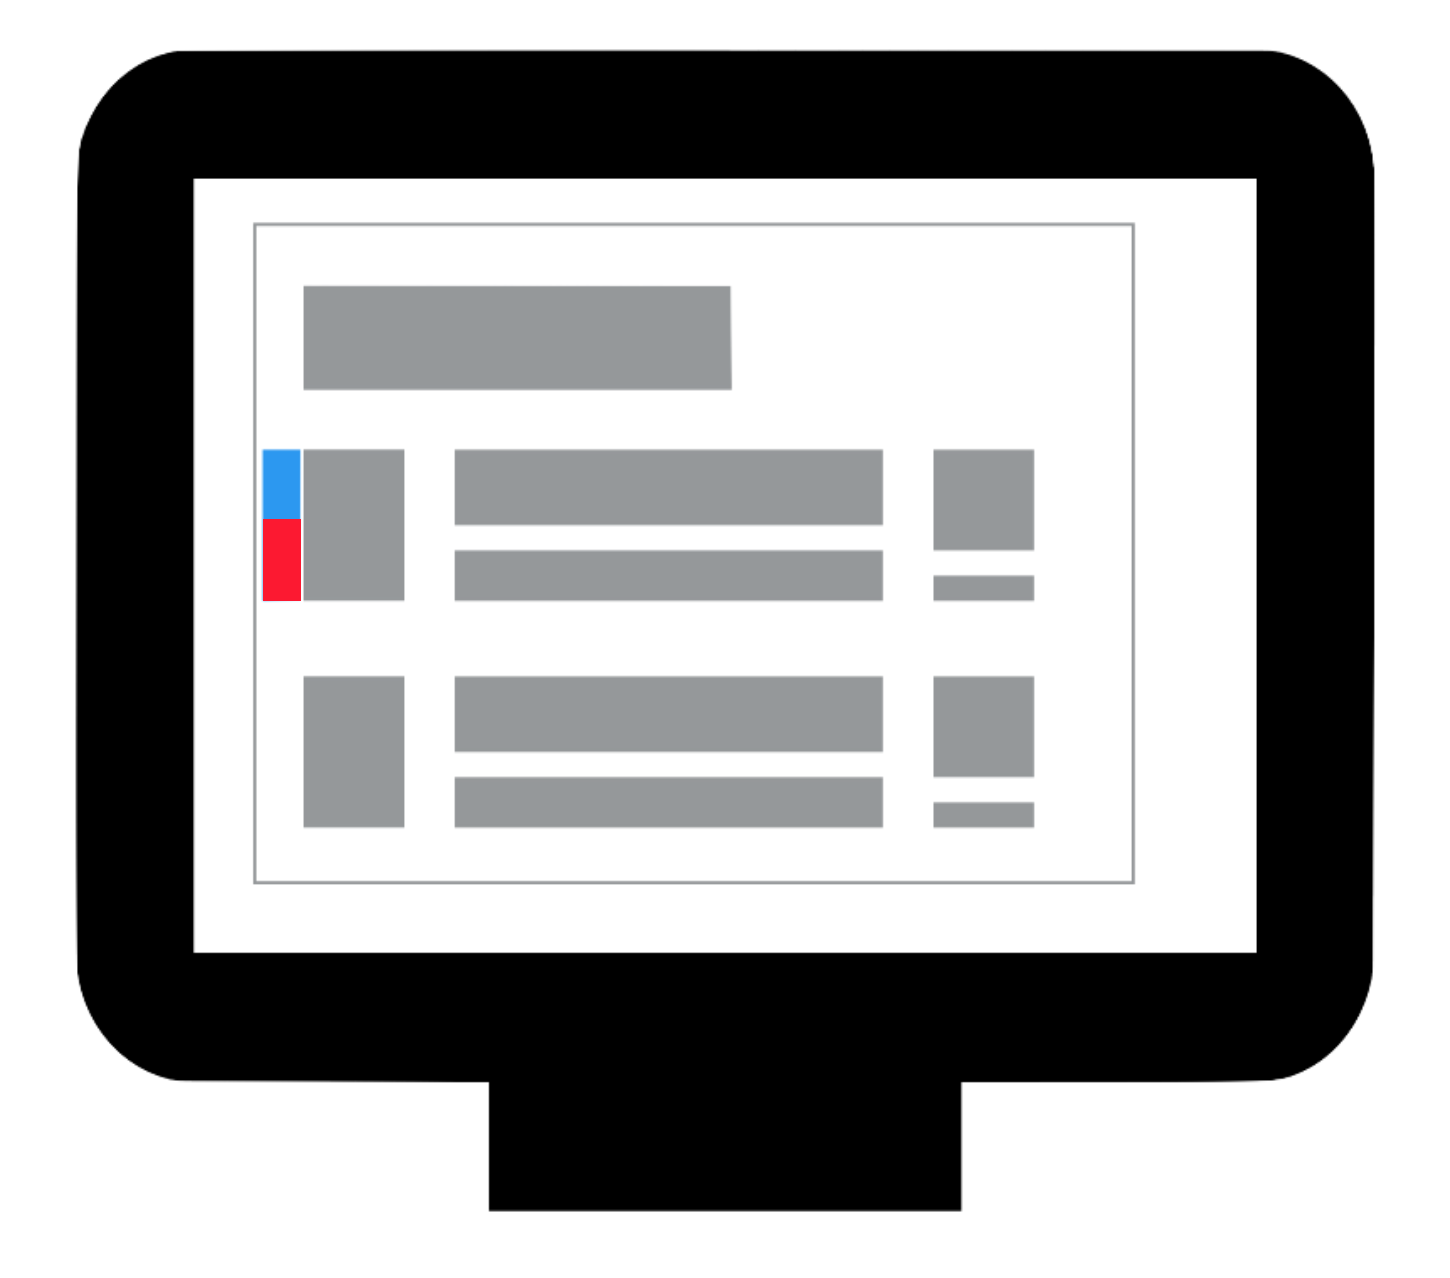
\includegraphics[width=0.4\textwidth]{./images/preference_colour/preference_splited}
  \caption{Preferences on display}

\end{figure}
\newpage
\section{Conclusion}
In this work, we proposed an architecture that supports users personalisation by creating two interactive applications. A \emph{Map Provider} web server provides a global overview of the state of beacons, displays and applications. Through its API is possible to dynamically link and unlink beacons to displays, manage applications and store basic users information. Our system supports realtime notification that is pushed into sockets and broadcasted to the clients updating their information accordingly. For example, if the display changes its running application then a message containing the new application is dispatched to the others devices in order to always provide a correct feedback to the user.

With a mobile application the viewers can both manage their preferences and discover applications. Specifically, it is possible to quickly enable and disable applications without changing the preferences related to them. Furthermore, a colour can be selected as preference's identifier. This information is stored into the \emph{Map Provider} and used as only way to recognise the owned content. Since only the creator knows the colour, then anonymity is maintained in the system.
Moreover, the mobile applications display real-time information about surrounding screens that have been discovered, such as the running applications.

In order to support users personalisation we develop two interactive applications: \emph{Transport} and \emph{Upcoming Classes}.
They implement the same interface providing a common API structure in order to be easily integrated into the system. 
\emph{Transport} allows users to select their bus schedules as preferences and to navigate content directly on the screen. For instance, it is possible to get the directions from the local display to one station, or to see the arriving buses timetable.
\emph{Upcoming Classes} shows the semester schedules supporting custom queries in order to discover specific content. It uses an event based calendar that supports both week and month views giving the ability to quickly discover all the schedules for a course. Each of them serves two single pages web application, one for the display, and one for the mobile application. They were developed using Vue.js a front-end framework that uses the paradigm of web components to create reusable code. Therefore, main of our code is shared across the applications.
All the applications support multi users model providing a \emph{non blocking} content flow where each user can discover information without been prevent by other viewers interactions. 

One key feature of the project is \emph{walk-by} contact personalisation. In this model, the users can pull its content into the system by just walking nearby a display in which a Bluetooth beacon is placed. The device is able to detect the mobile application's Bluetooth and dispatch its identifier in order to be discovered by the system. This methodology brings some advantages. For instance, it is not required to open the application nearby a display since it can run in background. 
One limitation is the hardware itself, we had some problems with the beacons. Since a connection delay is added by the manufacture to them, it may happen that a viewer has to wait some seconds before the mobile application is able to restore the connection with the beacon.

Since our system addres a heterogeneous audience, all the applications must be accessible. By keeping this consideration in mind we adopted a minimalistic content first design approach. In each UI the contents are showed into cards keeping logically clear the meaning of each component. Moreover, icons are widely used to provide a fast way to identify elements on the screen. In order to serve all the request from the same domain, a \emph{Proxy} was added to the system to avoid cross-origin requests.

In future work more applications and customisable preferences can be added. For example, an avatar could be also used to identify preferences on the screen. We also plan to integrate the proposed architecture into the current working university system. Due to the system scalability, deploying a new application is relatively easy since it only requires abstract constraints such as API endpoints design. Therefore, a new service can be implemented with any technology and host anywhere.
We strongly believe that public displays may become a new communication medium for the 21st century. With this project, we propose possible architecture design to supports users preferences that can be used as a starting point for future works.

%Displays are a powerful resource to reach a huge audience. Our architecture showed a way to implement custom users personalisation making them even more useful in a closed context such us this University. 
%
%We allows custom based preferences for the Lugano's public transportation giving the advantage to quickly see when a bus is leaving from a previously selected station. Also, the other application, shows the current semester schedules allowing a user to search for other courses.
%
%The preferences are managed using a mobile application served by the MAP Provider to, at the same time, know the global state of each display and access to all the services available. Also, is possible to disable the data flow on the fly for certainty applications allowing even more customisation and moving the control power to the user.
%
%In our University, a small environment compared to other well know the campus, walk-by contact personalisation really shines and proves is strong utility. Since the displays are deployed into key points such as \emph{Mensa} and \emph{Open Space}, users can easily access to them by just walking.

%%%%%
\newpage
\bibliographystyle{abbrv}
\bibliography{references}
\end{document}